%%%%%%%%%%%%%%%%%%%%%%%%%%%%%%%%%%%%%%%%%%%%%%%%%%%%%%%%%%%%%%%%%%%%%%%%%%%%%%%%
%2345678901234567890123456789012345678901234567890123456789012345678901234567890
%        1         2         3         4         5         6         7         8

\documentclass[letterpaper, 10 pt, conference]{ieeeconf}  % Comment this line out if you need a4paper

%\documentclass[a4paper, 10pt, conference]{ieeeconf}      % Use this line for a4 paper

\IEEEoverridecommandlockouts                              % This command is only needed if 
                                                          % you want to use the \thanks command

\overrideIEEEmargins                                      % Needed to meet printer requirements.

%In case you encounter the following error:
%Error 1010 The PDF file may be corrupt (unable to open PDF file) OR
%Error 1000 An error occurred while parsing a contents stream. Unable to analyze the PDF file.
%This is a known problem with pdfLaTeX conversion filter. The file cannot be opened with acrobat reader
%Please use one of the alternatives below to circumvent this error by uncommenting one or the other
%\pdfobjcompresslevel=0
%\pdfminorversion=4

% See the \addtolength command later in the file to balance the column lengths
% on the last page of the document

% The following packages can be found on http:\\www.ctan.org
%\usepackage{graphics} % for pdf, bitmapped graphics files
%\usepackage{epsfig} % for postscript graphics files
%\usepackage{mathptmx} % assumes new font selection scheme installed
%\usepackage{times} % assumes new font selection scheme installed
%\usepackage{amsmath} % assumes amsmath package installed
%\usepackage{amssymb}  % assumes amsmath package installed
\usepackage{multicol}
\usepackage{multirow}
\usepackage[bookmarks=true]{hyperref}
\usepackage{amssymb}
\usepackage{tabularx}
\usepackage{amsmath, mathtools, cuted}
\usepackage{algorithm2e}
%\usepackage{subfig}
\usepackage{caption}
\usepackage{subcaption}
\usepackage{float}
% \usepackage[]{footmisc}
% \usepackage{fancyhdr}
\usepackage[backend=bibtex,style=ieee]{biblatex}
\bibliography{references.bib}

\title{\LARGE \bf
%Language Guided Robotic Manipulation via Interpretable Programs}
%Learning Interpretable Programs for Language Guided \\ Neuro-Symbolic Robotic Manipulation}
%via Interpretable Programs}
%Learning Interpretable Programs for Language Guided \\ Neuro-Symbolic Robotic Manipulation}
Learning Neuro-symbolic Programs for Language Guided \\ Robot Manipulation}

\author{
Namasivayam K$^{*}$$^{1}$, 
Himanshu Singh$^{*}$$^{1}$, 
Vishal Bindal$^{*}$$^{1}$, 
Arnav Tuli$^{1}$, 
Vishwajeet Agrawal$^{\#}$$^{2}$, 
Rahul Jain$^{\#}$$^{2}$, \\
Parag Singla$^{1}$ and Rohan Paul$^{1}$\\
\small $^{1}$Affilitated with IIT Delhi. 
\small $^{2}$Work done when at IIT Delhi.
$^{*}$ and ${^{\#}}$ denote equal contribution.
}

% <-this % stops a space
% \thanks{$^{1}$Authors are with IIT Delhi. $^{*}$ and ${^{\#}}$ denote equal contribution.}


%\author{Albert Author$^{1}$ and Bernard D. Researcher$^{2}$% <-this % stops a space
%\thanks{*This work was not supported by any organization}% <-this % stops a space
%\thanks{$^{1}$Albert Author is with Faculty of Electrical Engineering, Mathematics and %Computer Science,
%        University of Twente, 7500 AE Enschede, The Netherlands
%        {\tt\small albert.author@papercept.net}}%
%}

\newcommand\parser{{\tt LanguageReasoner}}
\newcommand\sexec{{\tt VisualReasoner}}
\newcommand\dexec{{\tt ActionSimulator}}

\newcommand\percept{{\tt Perception}}
\newcommand\filter{{\tt Filter}}
\newcommand\action{{\tt Action}}

\newcommand\real{\mathbb{R}}
\usepackage{contour}
\usepackage{graphicx}
%\usepackage{ulem}
\usepackage{bbm}
%\renewcommand{\ULdepth}{1.8pt}
\contourlength{0.8pt}

\newcommand{\myuline}[1]{%
  \uline{\phantom{#1}}%
  \llap{\contour{white}{#1}}%
}

%Colors
\newcommand{\rohan}[1]{{\color{blue}{{#1}}}}
% \fancyhf{}%
% \renewcommand{\headrulewidth}{0pt}% No header rule
% \renewcommand{\footrulewidth}{0pt}
% \fancyfoot[L]{Accepted at International Conference on Robotics and Automation (ICRA),  2023 }%
% \pagestyle{empty}
\begin{document}



\maketitle
% \thispagestyle{fancy}%
\pagestyle{empty}

\begin{abstract}
%
%We present a neuro-symbolic model for learning robotic manipulation tasks. 
%
Given a natural language instruction and an input scene, our goal is to train a model %which when presented with a natural language instruction, and an input scene, 
to output a \emph{manipulation program} that can be executed by the robot.
%%, composed of learned actions and reasoning on the input scene, 
%describing how the input scene can be manipulated by the robot resulting in the intended scene. 
%
%The inferred program also provides sequential sub-goals as end-effector positions for the robot’s low-level motion planner to execute. 
%
Prior approaches for this task possess one of the following limitations: (i) rely on hand-coded symbols for concepts limiting generalization beyond those seen during training~\cite{paul2016efficient} (ii) infer action sequences from instructions but require dense sub-goal supervision~\cite{paxton2019prospection} or (iii) 
lack semantics required for deeper object-centric reasoning inherent in interpreting complex instructions~\cite{shridhar2022cliport}.
%
%From a modeling perspective, we first parse the natural language command in the form of a symbolic program, which is then executed over the input scene, using the neural representation of various symbolic concepts.
%
%The model learns grounded and executable neural representations for actions (as a transformation to objects in a latent space). 
%
% In contrast, our approach is neuro-symbolic and can handle linguistic as well as perceptual variations, is end-to-end differentiable requiring no intermediate supervision, and makes use of symbolic reasoning constructs which operate on a latent neural object-centric representation, allowing for deeper reasoning over the input scene.
In contrast, our approach can handle linguistic as well as perceptual variations, end-to-end trainable and requires no intermediate supervision. The proposed model uses symbolic reasoning constructs that operate on a latent neural object-centric representation, allowing for deeper reasoning over the input scene.
%, resulting in an expressive space of grounded manipulation programs.
%that are generalizable to unseen settings. 
%that are highly 
%interpretable and generalizable to unseen settings. 
%
Central to our approach is a modular structure  consisting of a {\em hierarchical instruction parser} and an {\em  action simulator} to learn  disentangled action representations.
%learned via RL and the use of \emph{gumble-softmax} layer to work as a selector facilitating \emph{disentanglement} in the action space. 
%
%Overall model is differentiable end-to-end with no intermediate supervision. 
%
%
Our experiments on a simulated environment with a 7-DOF manipulator, consisting of instructions with varying number of steps and scenes with different number of objects,  demonstrate that our model is robust to such variations and significantly outperforms baselines, particularly in the generalization settings. The code, dataset and experiment videos are available at \href{https://nsrmp.github.io/}{\texttt{https://nsrmp.github.io}} 
%the existing baseline.  
% Add: if we have the demo. 
%We also show a 7-dof manipulator using the model outputs to complete a stacking task involving sequential object interactions. 
\end{abstract}

\iffalse
% Earlier version
We address the problem of learning a model for neuro-symbolic robotic manipulation. Given the data in the form of triplets, with each triplet representing (a) a natural language instruction (b) an input scene, (c) an output scene, our goal is to train a model which when presented with a natural language instruction, and an input scene, can output a program (composed of learned actions and reasoning on the input scene), explaining how the input scene can be affected to result in the output scene. The inferred program also provides sequential sub-goals for the robot’s low-level motion planner to complete the intended task. 
Unlike previous approaches, which represent the program to be executed as a sequence of action labels ~\cite{paxton2019prospection}, our model works with explicit neural representation for actions (as a transformation to objects in a latent space), and is amenable to composition with pure symbolic reasoning. This makes our approach highly modular, interpretable, and generalizable to unseen settings. From a modeling perspective, we first parse the natural language command in the form of a symbolic program, which is then executed over the input scene, using the neural representation of various symbolic concepts. 
The key building blocks of our architecture include, training of the parser via reinforcement learning, and the use of \emph{gumbel-softmax} operation to work as a selector, while still allowing for back-propagation, facilitating disentanglement in the action space. The entire system is differentiable end-to-end with no intermediate supervision. Our experiments on a simulated environment, with commands consisting of variations, such as single actions, multiple actions, and scenes consisting of objects with varying attributes, demonstrate that our model is robust to all these variations, and outperforms a robust neural baseline.  
% Add: if we have the demo. 
%We also show a 7-dof manipulator using the model outputs to complete a stacking task involving sequential object interactions.
\fi

%\begin{abstract}
% version 1
%We address the problem of learning a model for neuro-symbolic robotic manipulation. Given the data in the form of triplets, with each triplet representing (a) a natural language instruction (b) an input scene, (c) an output scene, our goal is to train a model which when presented with a natural language instruction, and an input scene, can output a sequence of low-level robotic execution commands, represented as a program, to affect the desired manipulation, and result in the output scene. Unlike previous approaches, which represent the program to be executed as a sequence of action labels ~\cite{paxton2019prospection}, our model works with explicit neural representation for actions, as well as their arguments. This makes our approach highly modular, interpretable, and generalizable to unseen settings. From a modeling perspective, we first parse the natural language command in the form of a symbolic program, 
%with parser trained via reinforcement learning, 
%which is then executed over the input scene, using the neural representation of various symbolic concepts. 
%The key building blocks of our architecture include, training of the parser via reinforcement learning, and the use of gumble-softmax operation to work as a selector, while still allowing for back-propagation through symbolic representation. The entire system is differentiable end-to-end with no intermediate supervision. Our experiments on a simulated environment, with commands consisting of variations, such as single actions, multiple actions, and scenes consisting of objects with varying attributes, demonstrate that our model is robust to all these variations, and significantly outperforms the existing baselines by a huge performance margin.
%\end{abstract}

\section{Overview}

As robots enter human-centric environments, they must learn to act and achieve the intended goal based on natural language instructions from a human partner. The robot should be able to achieve this goal in different environments, with perceptual and lingual variation in environments and instructions it has seen before. We want to take a step towards building general robots which can be trained quickly in new environments, and can generalise well to complex instructions and scenes than what they have seen during training, necessitating them to have visuo-linguistic reasoning abilities. As the robots operate in novel environments without dependence on expert operators or users, they should learn with easily available data without fine-grained expert annotations.
%

We first address this problem of language-guided robot manipulation, which involves learning to translate high level language instructions into
executable programs grounded in the robot’s state and action space, and learning representations for visual and action concepts that can be composed to achieve the task.
%
We focus on multi-step manipulation tasks that involve object interactions such as stacking and assembling objects referred to by their attributes and spatial relations. 
%
We assume the presence of natural supervision from a human teacher in the form of input and output scenes, along with linguistic description for a high-level manipulation task. 
%
We also focus on making our approach interpretable, with an ability to reason and visualise the effects of actions before actually executing them.

We introduce a \textbf{neuro-symbolic approach} built on the concept learning framework by \cite{Mao2019NeuroSymbolic} for jointly learning representations for concepts that can be composed to form \emph{manipulation programs}: symbolic programs that explain how the world scene is likely to affected by the input instruction. The \emph{manipulation program} is grounded into the scene to get a sequence of actions that are fed to the low-level motion planner of the robot. 

For our study, we look at a table-top setting consisting of blocks of various types and colours, with instructions like \emph{"put the block which is behind the green dice to the right of the red cube"}, as can be seen in figure \ref{fig:example-nsrm}. The goal is to produce a high-level task plan consisting of a sequence of \textit{sub-goals} which a robot manipulator can execute, where each sub-goal consists of the knowledge of the object to be picked (i.e. a pick location) and its target position (i.e. a place location).
%

\begin{figure}
    \centering    \includegraphics[width=0.6\textwidth]{assets/example-nsrm.png}
    \caption{An example from our dataset, with the natural language instruction \emph{"put the block which is behind the green dice to the right of the red cube"}}
    \label{fig:example-nsrm}
\end{figure}

While the generated plans may be perfect in simulation, there are often marred by imperfections in the real world caused by noise in the sensory inputs, motor failures, or unexpected collisions. This results in deviations from the original path of planned execution, which the agent needs to recover from. An example can be seen in figure \ref{fig:error-example}, where the block falls off from the gripper mid-journey to the next sub goal. 

\begin{figure}
    \centering
    \begin{minipage}{0.3\textwidth}
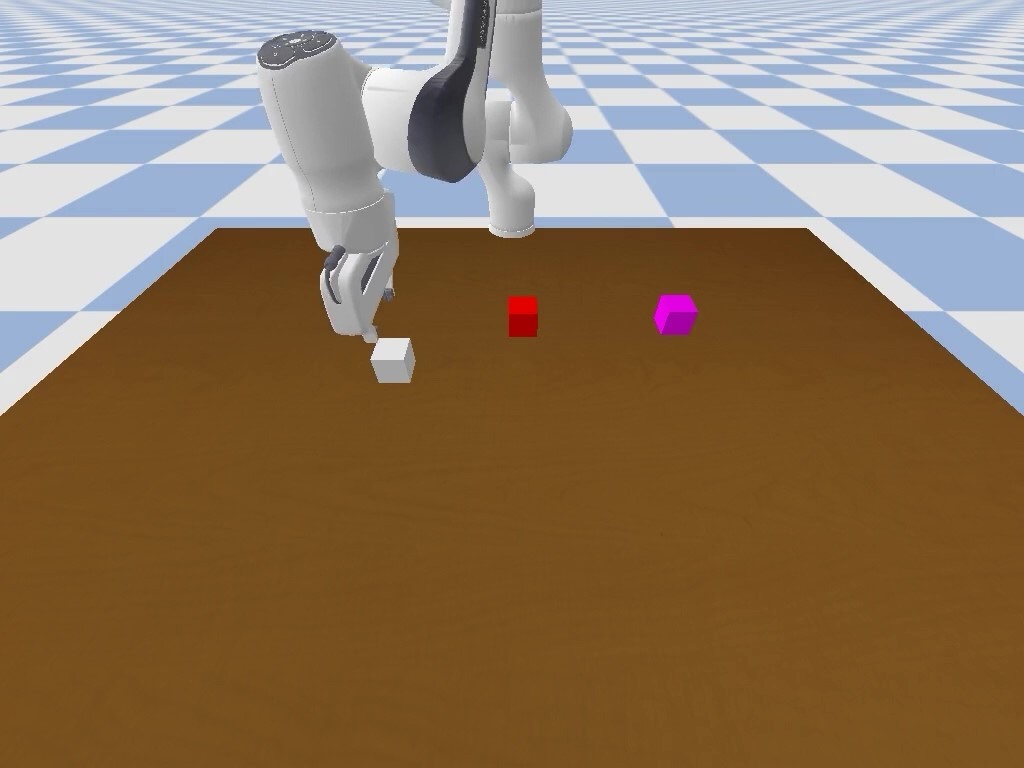
\includegraphics[trim={6cm 9cm 6cm 0},clip,width=0.9\textwidth]{assets/error-0.jpg}
    \end{minipage}
\begin{minipage}{0.3\textwidth}        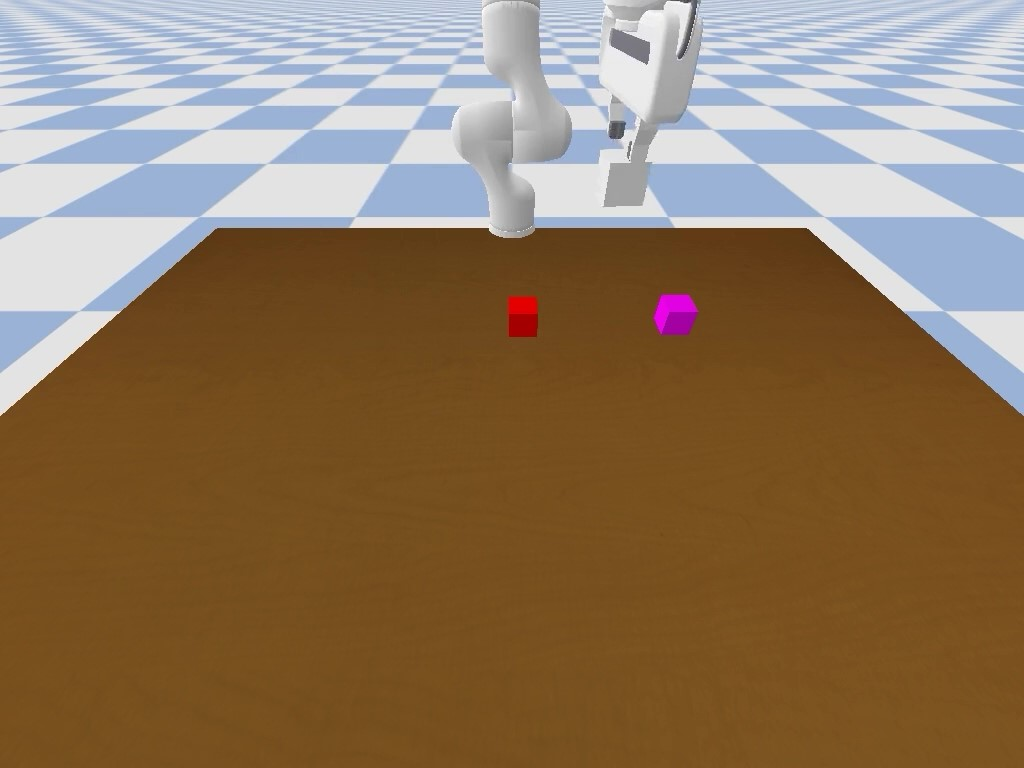
\includegraphics[trim={6cm 9cm 6cm 0},clip,width=0.9\textwidth]{assets/error-2.jpg}
    \end{minipage}
\begin{minipage}{0.3\textwidth}        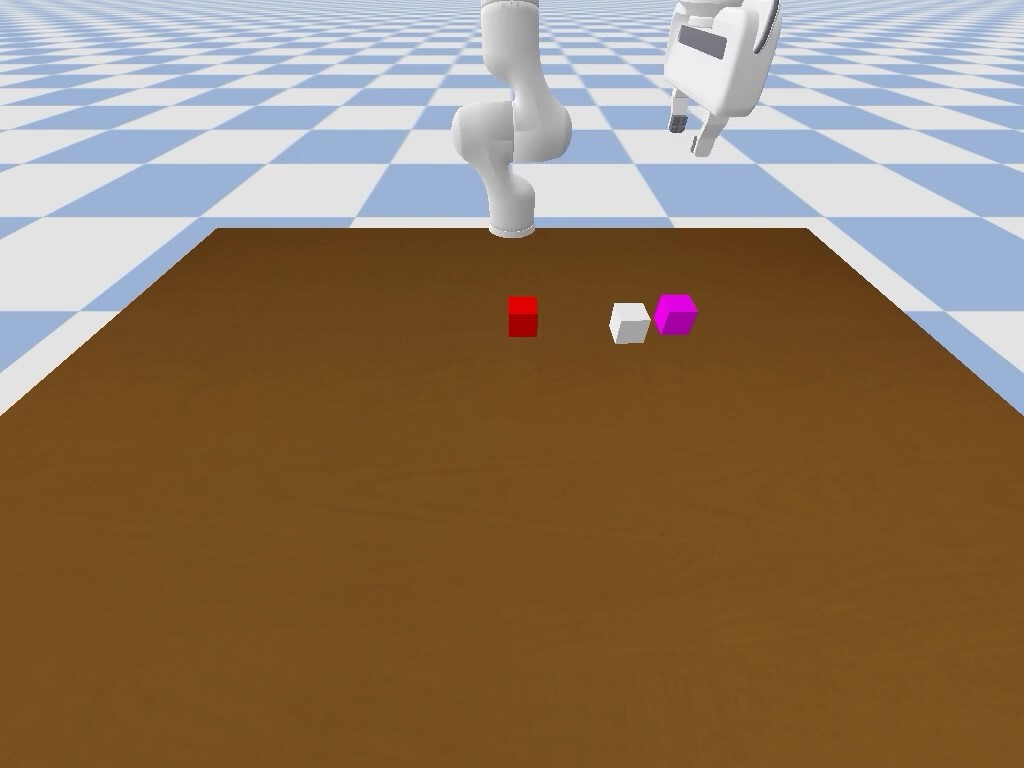
\includegraphics[trim={6cm 9cm 6cm 0},clip,width=0.9\textwidth]{assets/error-3.jpg}
    \end{minipage}
    \caption{Example of an execution error, due to a block falling off from the gripper. The original instruction was \emph{"put the white cube on top of the pink cube"}}.
    \label{fig:error-example}
\end{figure}

Often, the considerations of efficiency both in terms of time it takes to recover from the error, in terms of re-planning, as well as the time it takes for the new plan to reach the goal state, both become important. Further, even before recovery can happen, it is imperative that failures be correctly detected. We also note that this problem should be dealt without relying on hand annotated failure datasets, as they may be both time-consuming and expensive in terms of the human effort involved.  
%

Hence, our second goal is to build a scalable, self-supervised error detection and recovery mechanism which is efficiently able to detect discrepancies and reach the original goal while minimizing the time taken to re-plan. For our study, we simulate failures consisting of random external forces and perturbations of objects. We experiment with both single as well as multiple failures in a given plan. We introduce an efficient approach for \textbf{discrepancy-aware} failure-recovery mechanism based on an neuro-symbolic object-centric state representation.


\section{Problem Definition}

We thus address two problems in robot manipulation and task planning:

\textbf{Problem 1 [Learning Manipulation Programs]}: Given an initial world state and a natural language instruction, determine a sequence of sub-goals, which result in the final world state conforming to the instruction's intention.

The initial world state is given in the form of an RGBD image, and each sub-goal consists of the knowledge of the object to be manipulated and its target position. Only the final world state (as an RGBD image) is available for supervision during training. A DSL (Domain Specific Language) consisting of concept symbols is known, however their semantics are unknown. It is desired to achieve generalisation to novel scenes, instructions and plan lengths beyond those encountered during training, along with interpretability in sub-goals.

\textbf{Problem 2 [Error Detection and Recovery]}: For a robot manipulator executing a given plan on an initial world state, at each intermediate state, (i) determine if an error has occurred, and (ii) synthesise a plan to recover from the error so that the goal can be reached

For this problem, no addditional training data is assumed other than the data for the previous problem, specifically, no separate failure dataset is available for supervision. It is desired that the error recovery is quick, with minimal time taken for re-planning.

\section{Motivation}

The first problem of learning manipulation programs is hard since
\begin{enumerate}
    \item object attributes and actions have to be parsed from the underlying natural language sentence
    \item object references need to be grounded given the initial image.
    \item the effect of executing the specified actions has to be deciphered in the image space, requiring complex natural language as well as image level reasoning.
    \item The model needs to be trained end-to-end, learning representations for concepts via distant supervision.
    \item The approach needs to be interpretable and achieve generalisation to novel scenes and instructions
\end{enumerate}

Prior efforts for this problem can be broadly categorized as 
\begin{enumerate}
    \item Traditional methods which learn a mapping between phrases in the natural language to symbols representing robot state and actions in a pre-annotated dataset~\cite{howard2014natural,paul2016efficient,tellex2011approaching,matuszek2013learning,knepper2013ikeabot,gopalan2018sequence,williams2018learning}. They lack the flexibility to learn the semantics of concepts and actions on their own, which is an important aspect required for generalizability.
    \item Approaches that model an instruction as a sequence of action labels to be executed, without any deeper semantics, and requiring intermediate supervision for sub-goals, which may not be always be available~\cite{paxton2019prospection,shah2018bayesian,wang2020learning,kress2008translating,lazaro2019beyond,tenorth2010understanding,lisca2015towards,misra2016tell} 
    \item Recent end-to-end learning approaches~\cite{konidaris2018skills,wang2021learning, zettlemoyer2005learning,xia2018learning,silver2020few,zhu2021hierarchical,shridhar2022cliport,zeng2020transporter}; they have limited reasoning capability both at the level of instruction parsing, and their ability to learn varied action semantics.
\end{enumerate}

In response, our neuro-symbolic approach addresses these issues
\begin{enumerate}
    \item Our approach makes use of a Domain Specific Language (DSL) which specifies various concepts whose semantics are learned by the model. This allows generalizability to linguistic and perceptual variations in instructions and scenes respectively.
    \item The model is trained end-to-end and requires no intermediate sub-goal supervision. This allows training on easily obtainable form of data.
    \item Our latent neural object-centric representation allows for deeper reasoning needed to handle complex instructions and actions
\end{enumerate}
%

Prior works for the second problem on error recovery have been as follows

\begin{enumerate}
    \item Classical works have examined this problem in a purely symbolic setting, where the discovery simply corresponds to a goal check function, and recovery assumes the form of re-planning to the original goal, or repair to the sub-goal of last deviation from the plan.
    \item Alternate RL-based approaches learn a reactive policy that yield a high likelihood of reaching the goal from any state. However, they rely on well-enough offline exploration of the state space which is often difficult in complex manipulation domains.
    \item  More recently, literature has examined models which deal with perceptual data, containing various kind of noise, resulting in corresponding models for error recovery which account for variations in the input. Most approaches require hand annotated data sets, to learn a supervised function for discriminating two states from each other, both for error recovery, as well as re-planning. Creating such annotations, especially for failures, may be both time-consuming and expensive, in terms of the human effort involved. 
\end{enumerate}

%
In our work, we take a different approach to this problem, and ask the following question "Is there a way to learn a state discriminator function in a self-supervised manner which does not required hand annotated data for failed states?". An affirmative answer to this question would presumably help in building a scalable error recovery mechanism. Further, even after the failure has been detected, we would like to be efficiently able to reach the original goal while minimizing the time taken to re-plan, which can be prohibitive~\cite{fox2006plan}. This requires doing an efficient plan search to the desired sub-goal, which can exploit the localised information about where the failure might have occurred. 

Motivated by these questions, we propose an efficient approach for discrepancy aware failure recovery mechanism based on an object-centric scene-graph based state representation. 

\begin{itemize}
    \item Our state representation is decomposed in terms of individual object representations, which enables the agent to quickly discover what part of the state need to be changed to achieve the desired sub-goal, which is often the last state with correct execution of the original plan. 
    \item Central to our approach is a set of neural discriminators to separate out two different state as well as object representations trained in a self-supervised manner. Our discriminator not only detects failure, but also provides localised information about which objects have caused the failure by discriminating object representations.
    \item The search for recovery plan to the sub-goal, which is the last correct state, focuses on those objects which are the cause of the error as per the information provided by discriminator and manipulate these objects ignoring others. This results in a forward search accelerated with learned heuristics operating on a neuro-symbolic domain representation.
\end{itemize}


\section{Contributions}

For the first problem, our contributions are: 
%
\begin{enumerate}
\item A novel neuro-symbolic model that learns to perform complex object manipulation tasks requiring reasoning over scenes for a given natural language instruction and given initial world scene, without intermediate supervision.  
%
\item A CLEVR-like dataset for language-guided robot manipulation, consisting of a table top setting with a 7-DOF manipulator, blocks of various shapes and types, and language instructions with various levels of complexity.
%
\item Ability to interpret and visualise the model's latent program space by reconstructing any intermediate scene before execution by the manipulator 
%
\item Evaluation in instruction following experiments with a simulated robot manipulator, demonstrating robust generalization to novel settings improving on the state-of-the-art.
\end{enumerate}

This work is discussed in detail in chapter \ref{chap:part-1}. It was accepted at the International Conference on Robotics and Automation 2023 (\url{https://www.icra2023.org/}) as \\
\textbf{Learning Neuro-symbolic Programs for Language Guided
Robot Manipulation} \\
Namasivayam K$^{*}$, Himanshu Singh$^{*}$, \emph{Vishal Bindal$^{*}$}, Arnav Tuli, Vishwajeet Agrawal, Rahul Jain, Parag Singla, Rohan Paul

Information regarding the paper, video and code is at \url{https://nsrmp.github.io/} 


 For the second problem, our contributions are:
 \begin{enumerate}
     \item An efficient approach for discrepancy-aware failure detection and recovery, based on a neuro-symbolic state representation
     \item Neural modules for state transition and discrimination learned without any additional failure datasets
     \item A recovery mechanism consisting of forward search guided with learned heuristics
     \item Evaluation with various degrees of simulated errors, demonstrating strong improvement over baselines in terms of time taken for error recovery
 \end{enumerate}

 This work is discussed in detail in chapter \ref{chap:part-2}. It is currently under review at Conference on Robot Learning 2023 (\url{https://www.corl2023.org/}) as \\
 \textbf{Learning to Recover from Plan Failures using Fast Discrepancy-Aware Neuro-Symbolic Search} \\
 Arnav Tuli$^{*}$, \emph{Vishal Bindal$^{*}$}, Namasivayam K, Himanshu Singh, Parag Singla, Rohan Paul

\textbf{Grounding Instructions to Robot Control.} Traditional approaches for grounding instructions assume a symbolic description of the environment state 
and robot actions. 
%
These approaches learn to associate phrases in an instruction with symbols conveying their meaning from 
annotated datasets. 
%
For example, \cite{howard2014natural,paul2016efficient,tellex2011approaching} map language to discrete motion constraints that can be provided to a motion planner for trajectory generation, \cite{matuszek2013learning,knepper2013ikeabot} parse language to a logical parse that includes  robot control actions and \cite{gopalan2018sequence,williams2018learning} use sequence to sequence modeling to ground language to LTL formulae capturing high-level task specifications. 
%
% Such approaches assume a symbolic model of the world (either hand coded or a-priori learned). 
% The approach presented in this work, additionally learns dense disentangled representations for 
% spatial concepts as well as actions from data while learning a grounding for an input instruction.  
%
In contrast to such approaches, the proposed work doesn't assume a symbolic model of the world and learns spatial and visual concepts and action semantics from data. 

\textbf{Inferring Plans from Instructions.} Another set of approaches focus on multi-stage tasks (e.g., cooking, assembly etc.) and propose 
learners that can infer action sequences by observing human task demonstrations. 
%
The work in ~\cite{paxton2019prospection} proposes a recurrent neural architecture that converts a natural language instruction to a sequence of intermediate goals for robot execution. 
%
Efforts such as \cite{shah2018bayesian,wang2020learning,kress2008translating} learn LTL task specifications from humans demonstrations and introduce a model for effectively searching in the space of programs. 
%
In another effort, ~\cite{lazaro2019beyond}, authors introduce a cognitively-inspired approach that infers 
a likely program from a symbolic generative grammar for a robot manipulator to form and re-arrange block patterns
in a table top setting. 
%
% Tenorth et al. \cite{tenorth2010understanding,lisca2015towards} use human activity demonstrations to train a relational probabilistic model to infer fully grounded symbolic plans from instructions. 
%
Misra et al. \cite{misra2016tell} present a similar approach but additionally assess plan feasibility for inferred plan candidates 
using a symbolic planner in the training loop. 
%
Despite successful demonstrations, these approaches require dense  
intermediate supervision and treat robot actions in a purely symbolic manner without learning their deep grounded semantics. 
%
% The proposed method learns a latent space of grounded programs which can be executed in the latent space of object representations. The explicitly reason with disentangled and modular concepts enables learning from \emph{only} the initial and final state data, forgoing the need for dense intermediate supervision. 
However, our method learns a latent space of composable symbolic programs which can be executed in the latent space of object representations. The composability of the  symbolic programs enables incremental learning through a specified curriculum from only the initial and final state data, forgoing the need for dense intermediate supervision. 


\textbf{Learning Action Models.} This work builds on the rich literature on acquiring action models for planning and captures \emph{when} actions are applicable and 
\emph{how} they affect the world. 
%
Efforts such as \cite{konidaris2018skills} and \cite{wang2021learning} 
learn initiation sets for actions implicitly learning to classify
the robot's configuration space where an action can be initiated. 
%
% Hannah et al. ~\cite{zettlemoyer2005learning} address the complementary problem of acquiring the 
% transition model and present an algorithm for determining \emph{planning rules} expressing 
% possible symbolic states resulting from the robot performing an action. 
%
~\cite{xia2018learning,silver2020few,zhu2021hierarchical} present neuro-symbolic approaches for learning a latent object-centric world model for tasks such as stacking, re-arrangement etc.  
%
In \cite{shridhar2022cliport}, authors introduce an end-to-end model that jointly predicts object affordances  and object displacements specifying metric goals for robot re-arrangement and sorting tasks. 
%
Recent parallel work by Wang et al. \cite{wang2023programmatically} builds on \cite{shridhar2022cliport} and represents the task as an executable program parsed from the instruction using a CCG parser, restricting the length and variation of the instructions it can handle. 
% 
Even though these approaches successfully learn modular action models that are amenable to planning, the scope of reasoning is limited to one-hop reasoning over spatial relations and attributes. In contrast, this work focuses on interpreting task instructions that require compositional/hierarchical spatial reasoning over an extended planning horizon. 



%% %%%
\iffalse

\textbf{Robot Skill Learning. }
The ability to reason and plan tasks is conditioned on the robot possessing knowledge 
of when it can perform actions and how it affects the world. 
%
Traditional approaches such as~\cite{knepper2013ikeabot} 
model robot actions as symbolic pre-conditions and effects. 
%
Such representations are often hand-coded making them 
brittle and error-prone in practice. 
%
Learning based efforts aim at acquiring actions representations through human demonstration 
or via self-supervision. 
%


\textbf{Robot Task Planning and Representations. }
Instead of focusing on learning primitive skills, complementary efforts have 
focused learning to translate a high-level instruction to a sequence of symbolic actions 
to accomplish multi-step tasks such as navigation or assembly. 

In ~\cite{paxton2019prospection}, authors introduce a recurrent architecture that 
translates language instructions into a sequence of sub-goals for the manipulator to follow. 
Central to the approach is a recurrent architecture that learns to predict sequential changes in the world 
model caused by robot actions. Although the model makes significant progress in predicting future world states, 
the model lacks the notion of grounded and executable representation for actions. As a result, 
the generalization performance degrades with tasks possessing repetitive structure that are unseen in training. 

The work in  ~\cite{paxton2019prospection} tackles the problem of learning spatial relational concepts 
and introduce a neural model that uses a bottleneck layer to recover disentangled representation for action. 
The task of converting an instruction to a sequence of symbolic actions is largely treated as sequence to 
sequence problem. Such a representation limits scope for rich reasoning and generalization to novel scenes.  
%
In contrast, this work adopts a program learning view, with explicit grounded representations for manipulation 
concepts that can be composed in symbolic programs allowing explicit reasoning with learned neural modules. 

In another effort, ~\cite{lazaro2019beyond}, authors introduce a cognitively-inspired approach for inferring 
executable programs. The authors demonstrate the ability to recover programs that the robot can execute to
modify block patterns to a target configuration. However, the authors assume a deterministic grounding from 
sensory inputs to discrete symbols. In contrast, this work builds an action representation directly on the 
perceived objects in the manipulation area. 


Finally, other efforts have attempted to learn rich logical description of tasks from human demonstration 
aimed towards inductive generalization to novel domains. 
%
 
 %
In contrast, this paper learns executable concepts that can be reasoned when combined in programs, 
endowing the ability to synthesize the world state after program execution.  
%
%Similarly, introduce a policy prior that effectively constrains the program space. 

\textbf{Instruction Following. }
Related efforts address the problem of inferring manipulation constraints \cite{howard2014natural, paul2016efficient} 
that that capture the intended goal from language utterance for the purposes of commanding a robot. 
%
Prominent models such as learn to associate linguistic constituents with a symbolic representation of the environment. 
%
The likely association or the \emph{grounding} for the instruction is used to derive a motion plan for the robot. 
%
Such approaches assume the presence of spatial concepts and focus on learning the association between language 
and they physical world state. 
%
The work presented in this paper, learns such spatial and action concepts directly from natural supervision forgoing the need 
for explicit hand coding of concepts. 
%
Other related efforts \cite{paul2018temporal, roy2019leveraging} 
learn groundings for actions and spatial relations assuming a set of hand-coded features 
or directly from data but lack an explicit representation of symbolic reasoning which may be needed for interpreting 
an instruction. 
%
The explicit notion of a program space used in this work makes learned grounded concepts amenable 
to symbolic reasoning.  
%

 
\textbf{Neuro-symbolic concept learning. } 
%
This paper builds on the Neuro-symbolic concept learning framework~\cite{Mao2019NeuroSymbolic}. 
The ability to acquire executable concepts from natural supervision. Applied to the visual question answering task. 
%
These approaches have successfully demonstrated the ability to learn static spatial concepts (relative positions, orientations)
and image attributes such as (appearance) etc. 
%
Recent efforts such as ~\cite{yi2019clevrer}, model dynamic interactions such as collisions an additionally model object consistency 
using temporally consistent appearance cues. 
%
We build on the model introduced in ~\cite{Mao2019NeuroSymbolic}. 
%
This work introduces the physical agent affecting the scene and 
address the task of learning grounded and executable representations for robot actions that cause changes in the 
environment in service of symbolic goals such as creating assemblies. 
%
More generally, neuro-symbolic approaches have also found applications in visual-question answering~\cite{yi2018neural}, 
modeling visual structure in scenes~\cite{li2020multi}, inferring motion programs~\cite{kulal2021hierarchical} etc.  
%
%To the best of our knowledge, the task of learning action representations for goal-directed physical agent affecting the environment 
%has not been addressed. 
% 

\fi


\label{sec:problem2}
%% Planning Model Figure

\begin{figure}
    \begin{subfigure}{1.0\hsize}
         \centering    
         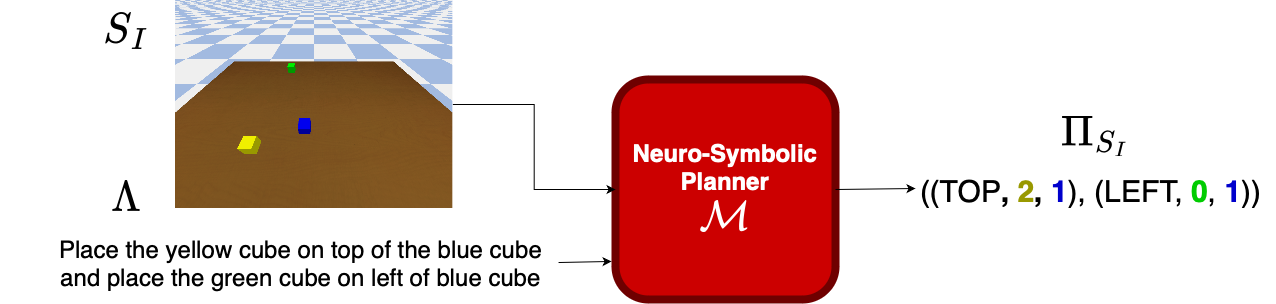
\includegraphics[scale=0.25]{figures/nsrm.png}
    \end{subfigure}
    \caption{
        % \footnotesize{
            \textbf{Planning model.} 
            This work assumes a planning model that given a language utterance and the current world state can synthesize a sequence of actions for manipulation tasks. Crucially, the actions (as well as spatial relations) are functions that can be trained from goal-reaching human task demonstrations. 
        }
    % }
    % \vspace{-0.15in}
    \label{fig:nsrm}
\end{figure}

\begin{figure}
    \centering
    \begin{subfigure}{.45\textwidth}
        \centering
        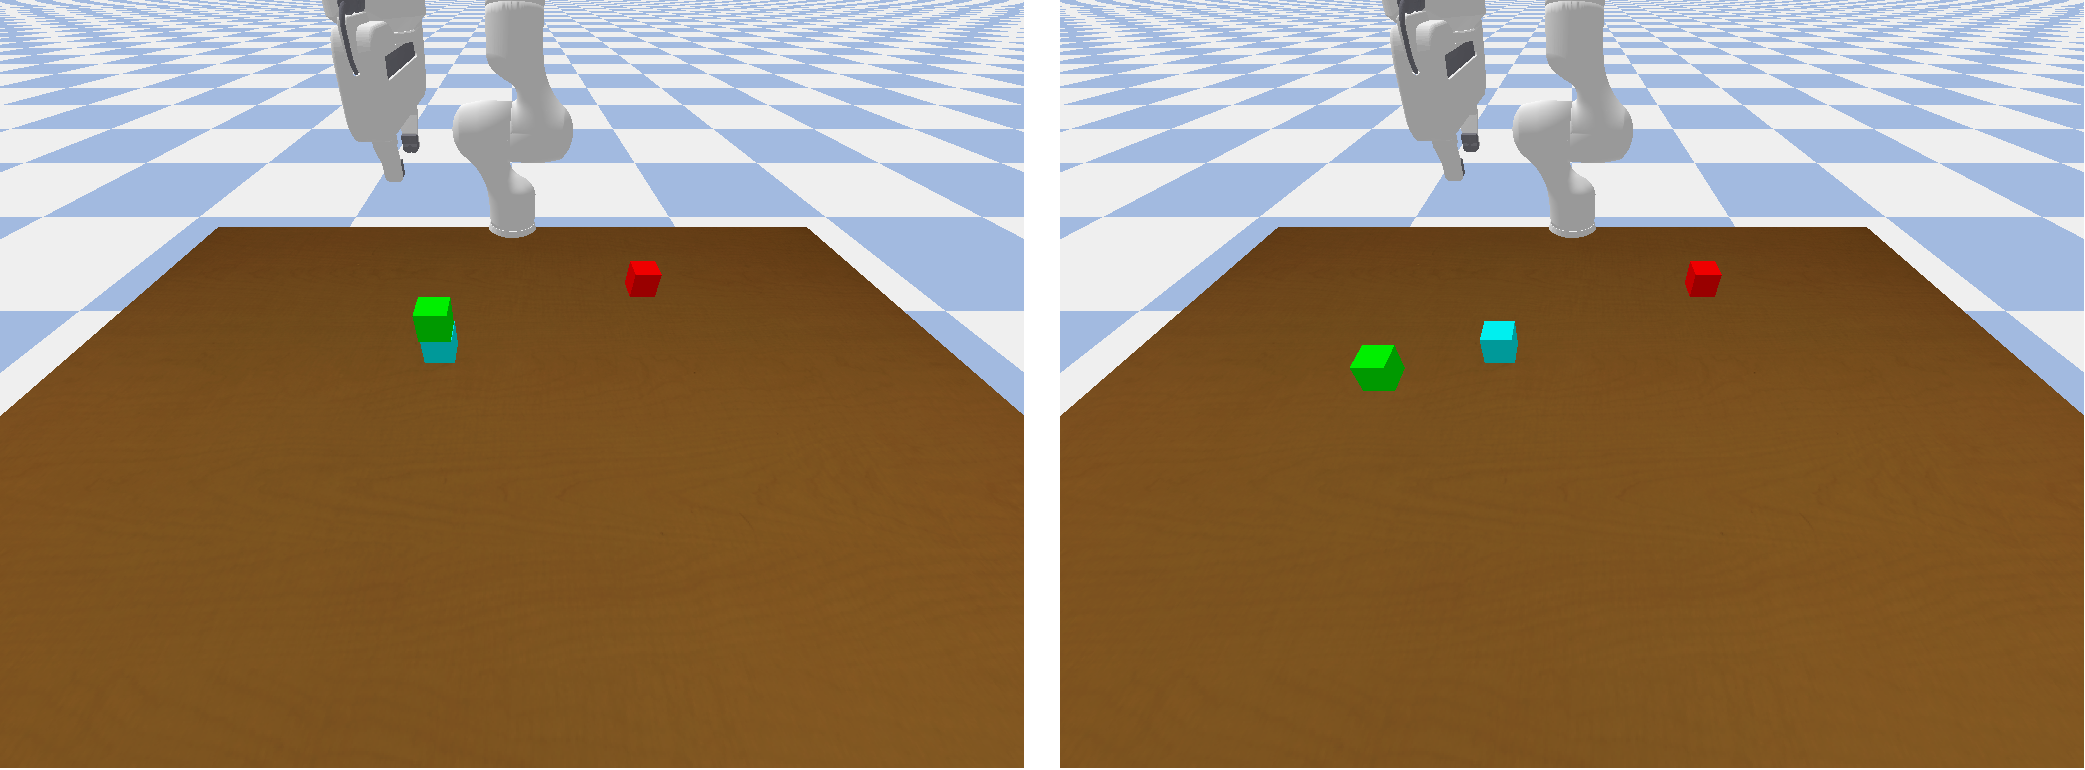
\includegraphics[width=\textwidth]{assets/error-force.png}
        \caption{External force on \\green cube}
    \end{subfigure}
    \hfill
    \begin{subfigure}{.45\textwidth}
        \centering
        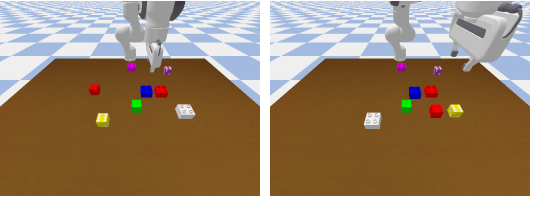
\includegraphics[width=\textwidth]{assets/error-interchange.png}
        \caption{Interchange of yellow dice and white lego by an external agent}
    \end{subfigure}

    \vspace{1cm}

    \begin{subfigure}{.45\textwidth}
        \centering
        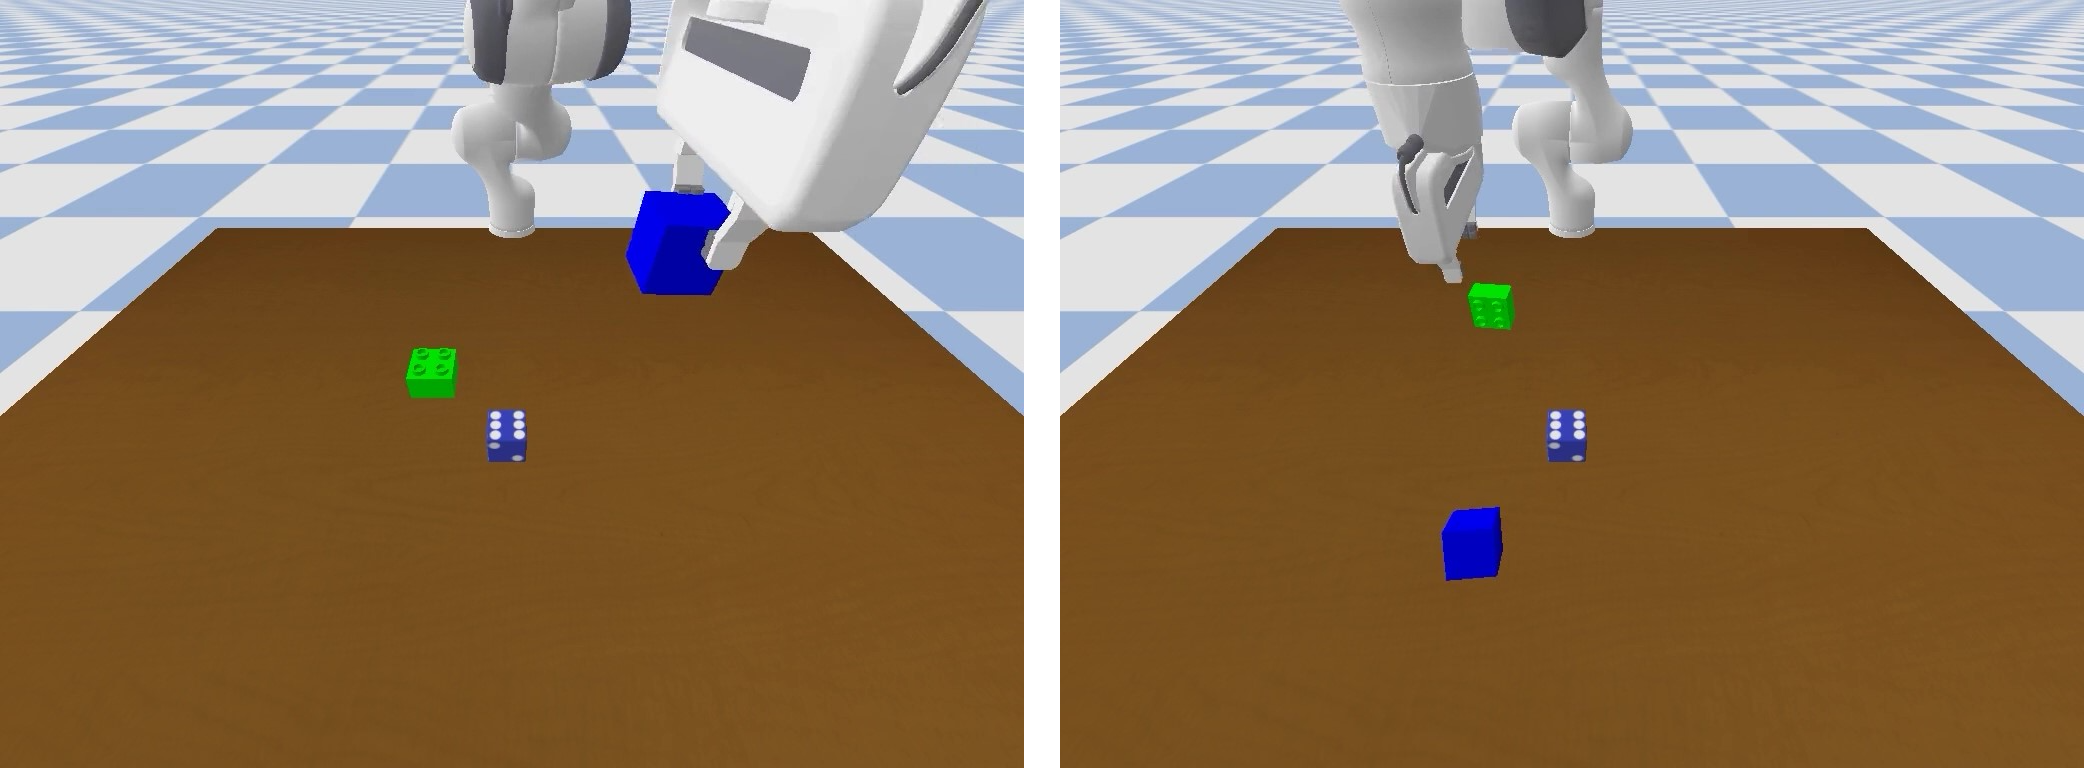
\includegraphics[width=\textwidth]{assets/error-gripper.png}
        \caption{Gripper error leading to falling blue cube displacing underlying green lego}
    \end{subfigure}
    
    \caption{Various possible errors during robot execution}
    \label{fig:errors-possible}
\end{figure}


\textbf{Robot Model. }
Consider a robot manipulator capable of grasping and releasing objects in a table-top workspace. 
%
The robot can be tasked with instructions such as ``place the green block on top of the red object and the yellow block on top of the green one" that require the robot to sequentially manipulate objects to achieve an intended block assembly. 
%
We assume that the robot perceives the world through the visual sensor and is equipped with a primitive skill for grasping a specified object and releasing it at a given pose on the table or on another object. 
%
Further, we assume the presence of a planning model, $\mathcal{M}$, which given an initial world state $S_I$ and a goal specified as a language utterance $\mathit{\Lambda}$, can synthesise a plan $\mathbf{\Pi_{S_I}}$ for the robot to execute. 
%
Here, the plan $\Pi \in \mathcal{P}$ is a sequence of $T$ symbolic actions $\Pi = (\pi_1, \pi_2, .., \pi_T)$. The state $S_I$ is assumed to be represented as a set of bounding boxes extracted from a visual and depth sensor using a pre-trained object detection model. 

%
\textbf{Planning Model. }
%
We build on~\citep{Kalithasan2022LearningNP}, a contemporary neuro-symbolic planner that can learn grounded models for spatial concepts (left, right, on top etc.) as well as actions (e.g, moving an object to a prescribed location). 
%
The planner (Figure~\ref{fig:nsrm}) outputs a sequence of triplets ($a_t$, $o_{1t}$, $o_{2t}$), where $a_t$ is the symbolic action and, $o_{1t}$ and $o_{2t}$ are the indices of the \textit{subject} and \textit{object} of the manipulation task respectively. 
%
The predicted state changes by executing a plan $\mathbf{\Pi} \in \mathcal{P}$ on the state $S \in \mathcal{S}$ is modeled as a function, $\mathcal{E}: \mathcal{S} \times \mathcal{P} \rightarrow \mathcal{S}$. 
%
Further, let $\mathcal{K}: \mathcal{S} \times \mathcal{A} \rightarrow \mathcal{S}$, denote the \emph{transition model} that determines the state resulting from taking an action in a given state under nominal conditions (without errors). The transition model  $\mathcal{K}$ expresses the function $\mathcal{E}$ as follows where the state $\mathcal{E}(S, \mathbf{\Pi})$ will be reached if the plan is executed by the robot without any errors. 
%
\begin{equation}
    \mathcal{E}(S, \Pi) = \mathcal{E}(\mathcal{K}(S, \pi_1), (\pi_2, \pi_3, \dots, \pi_T)),
\end{equation}

% ROLL OUT FIGURE
\begin{figure}
    % \begin{subfigure}{1.0\hsize}
         \centering     \includegraphics[width=\textwidth]{figures/demo.png}
    % \end{subfigure}
    \caption{
            \textbf{Error detection and recovery pipeline.}
             Using the scene-graph predictor, we can \textit{imagine} the intermediate states that the robot should encounter during manipulation. We compare those with the actual state at run-time (at each step) and detect discrepancies if any. In case of discrepancy, our recovery mechanism kicks in and a plan is generated to the \textit{imagined} state. 
    }
    % \vspace{-0.15in}
    \label{fig:rollout}
\end{figure}

\textbf{Learning to Recover Plans. }
%
Online plan execution may be prone to \emph{internal} or \emph{external} disturbances, causing the robot to be in an \emph{unplanned} erroneous intermediate state, $S_E$. See figure~\ref{fig:errors-possible} for examples of such disturbances.  Hence, the robot may find itself in intermediate states to be different than the ones expected $S_t$ due to disturbances which necessitates the synthesis of a new \emph{recovery} plan $\mathbf{\Pi_{S_E}}$, such that $\mathcal{E}(S_E, \mathbf{\Pi_{S_E}}) =_\mathcal{S} \mathcal{E}(S_I, \mathbf{\Pi_{S_I}})$, see Figure~\ref{fig:rollout}.
%
Formally, for each $t \leq T$, we inductively define $S_t = \mathcal{K}(S_{t - 1}, \pi_t)$, where $S_0$ is the initial state. These $S_t$'s represent the \emph{intended} intermediate states for the robot. Further, let the states encountered during \emph{actual} execution be $S'_t$, $t \leq T$. 
%
The relation $=_\mathcal{S}$ on $\mathcal{S}$ holds if and only if the 3D positions of the corresponding objects in the two states are within some $\delta$ threshold. 
%
A plan recovery model requires addressing the following. First, estimating if there is a plan error (or discrepancy) as whether $S'_t =_\mathcal{S} S_t$ before executing action $\pi_{t + 1}$, for all plan execution steps $t$. 
%
Second, if a discrepancy is estimated, then synthesize a plan $\mathbf{\Pi_{E(t)}}$ such that $\mathcal{E}(S'_t, \mathbf{\Pi_{E(t)}}) =_\mathcal{S} S_k$ for some $k \leq T$.
%
Further, append the sequence $(\pi_{k + 1}, \pi_{k + 2}, .., \pi_T)$ to $\Pi_{E(t)}$ to get the overall plan $\Pi_{S_t'}$, such that $\mathcal{E}(S_t', \Pi_{S_t'}) =_\mathcal{S} S_T$. 

We propose a neuro-symbolic architecture to solve the task planning problem described in section \ref{sec:problem}. Our architecture is inspired by ~\cite{Mao2019NeuroSymbolic} and is trained end-to-end with no intermediate supervision.
%
We assume that the reasoning required to infer the sub-goals can be represented as a program determined by a domain specific language (DSL). Table \ref{table:dsl} lists the keywords and operators in our DSL, along with the implementation details of the operators. We assume a lexer that identifies all the keywords that are referred to in the  instruction $\Lambda$. We do not assume prior knowledge of the semantics of the DSL constructs, and they are learned purely from the data.
%
Our architecture (ref. Figure~\ref{fig:schematic}) consists of the following key modules (a) Language Reasoner (LR) to parse the instruction into a hierarchical plan consisting of references to visual and action concepts and operators (b) Visual Extractor (VE) to obtain the initial bounding boxes from the input image (c) Visual Reasoner (VR) to ground the object related concepts present in the parsed instruction with respect to the input image (d) Action Simulator (AS) to learn the semantics of actions to be executed to produce a sequence of sub-goals. Figure ~\ref{fig:approach} illustrates our approach. \ref{fig:approach-1} shows the output of executing the emboldened sub-tree on the input scene. In \ref{fig:approach-2}, the visual reasoner computes the grounded program from the symbolic program generated by the language reasoner. The grounded program is used by the action simulator to compute the final location of the moved object. This is fed into a low-level motion planner for computing the low-level trajectory.

\begin{figure}
    \centering 
    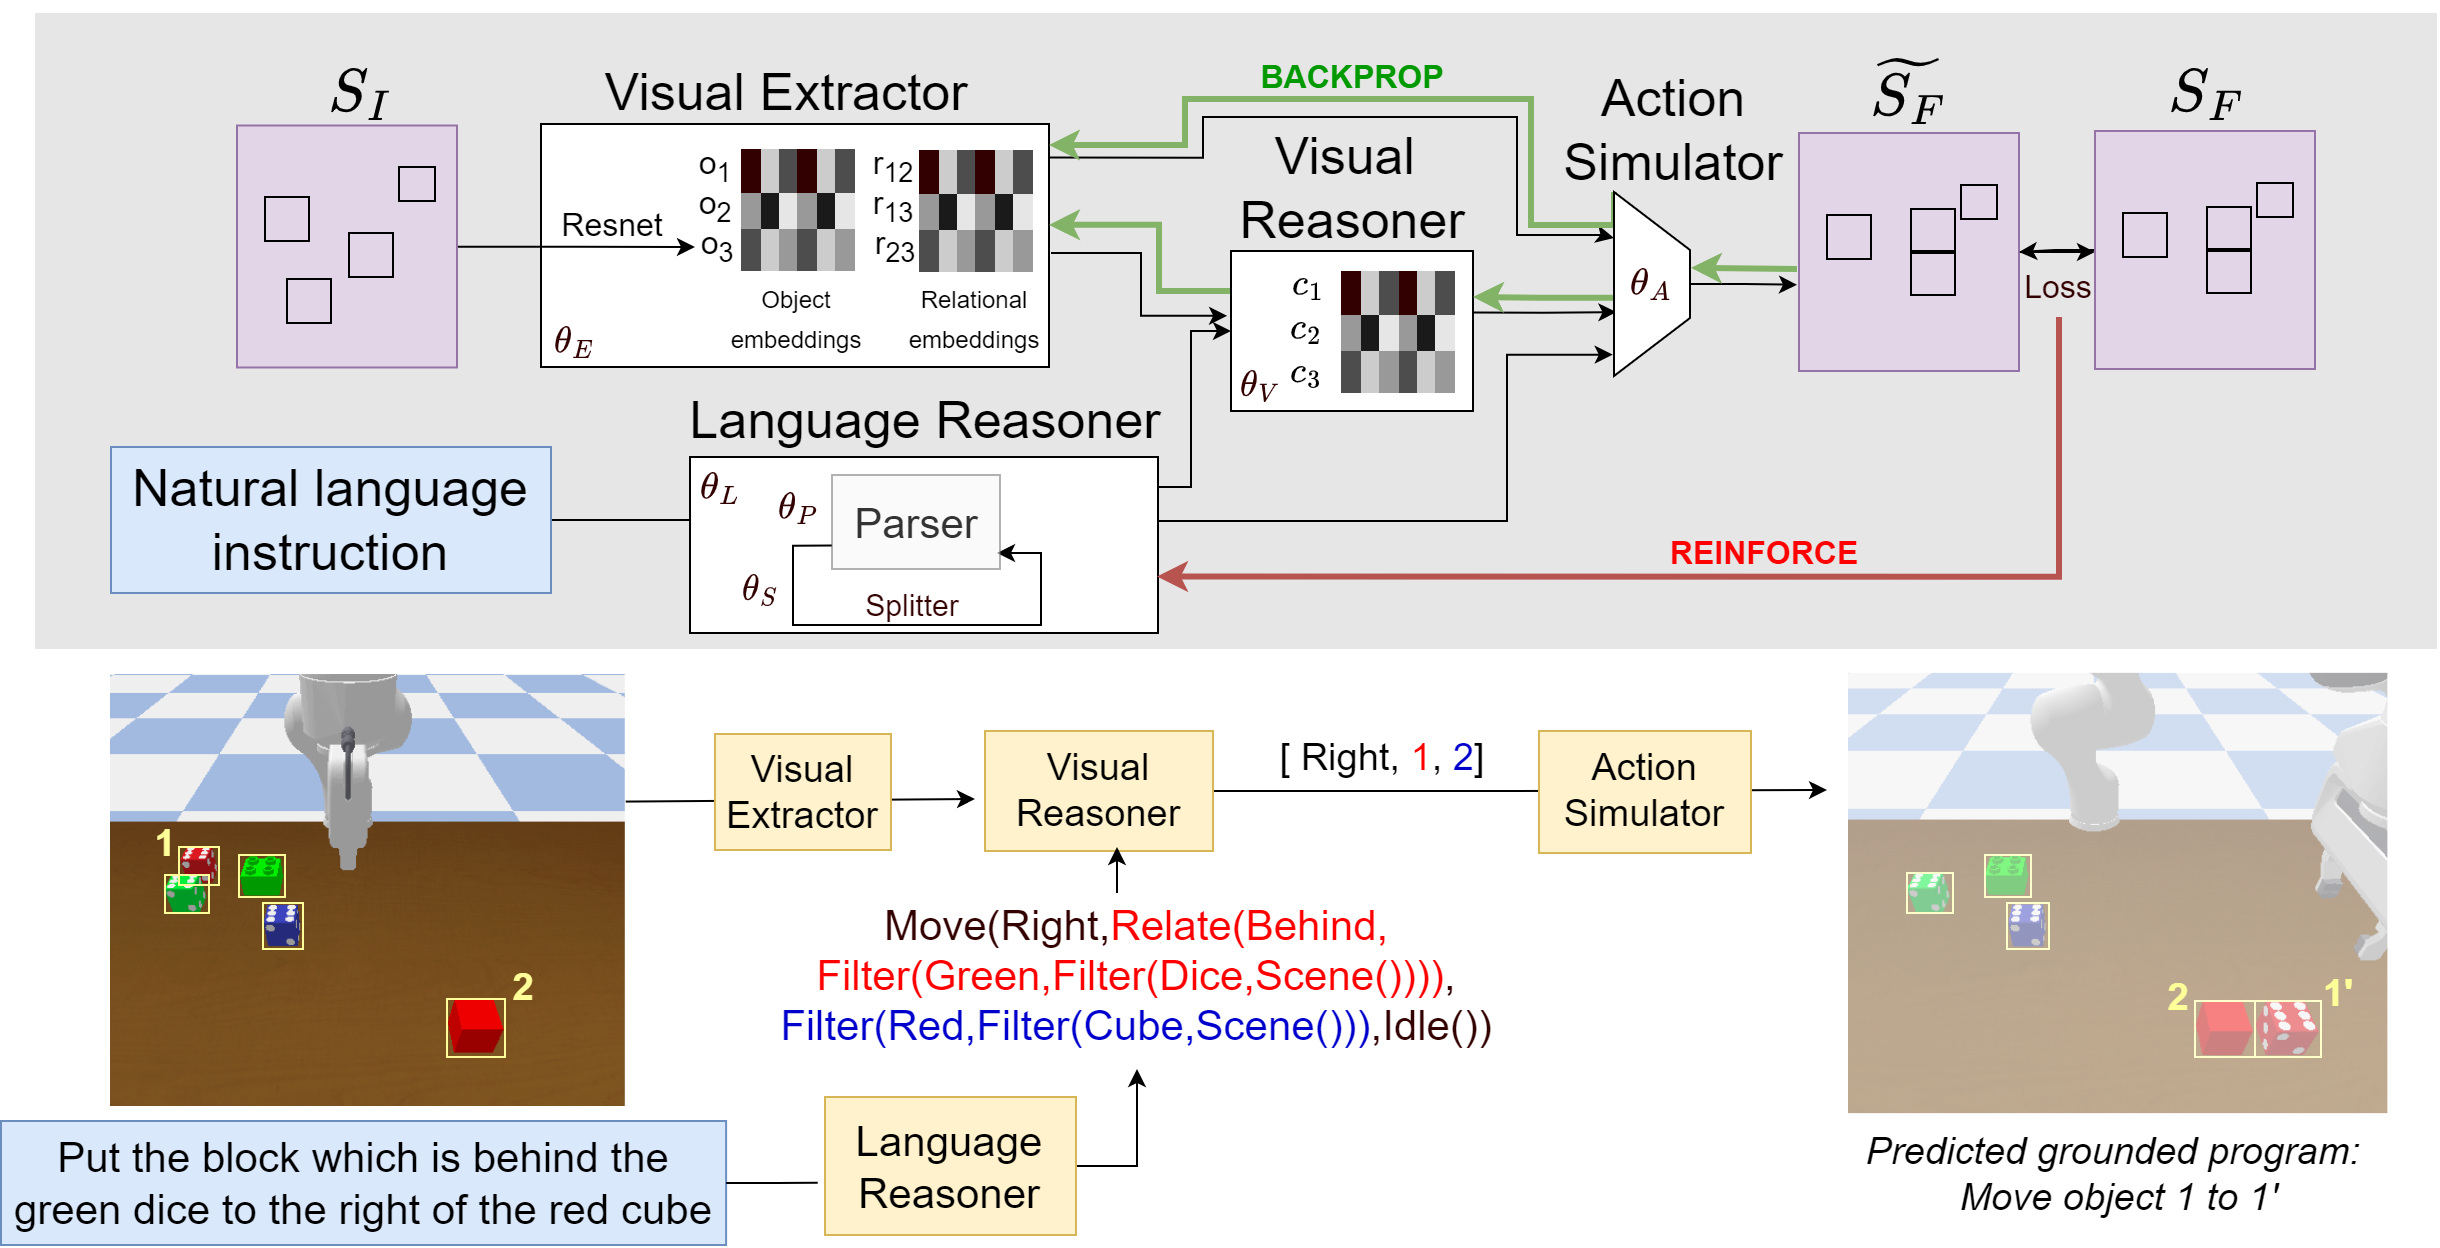
\includegraphics[width=\textwidth,clip,trim={0 20.5cm 0 0}]{figures/main-model-3.png}
    \caption{Neuro-symbolic Model architecture for learning manipulation programs}
    \label{fig:schematic}
\end{figure}

Unlike ~\cite{Mao2019NeuroSymbolic}, where the program execution is purely symbolic and deterministic, the program execution in our case is also neuro-symbolic. This brings difficulty in training the LR, but enables us learn the sub-goal generation. 
Finally, we also provide an encoder to extract objects from the initial scene $\tilde{S}_I$ , and a decoder to construct the final scene, $\tilde{S}_F$, once the sub-goals have been executed.


\begin{table}
    \centering
    \begin{tabular}{|p|p|p|p|}
    % \begin{tabular}{|p{0.01cm}|p{0.01cm}|p{0.08cm}|p{0.08cm}|}
        \hline
        \multicolumn{4}{|c|}{\textbf{Keywords and their classes}}\\
        \hline
         \multicolumn{2}{|c|}{\textbf{Object-level concepts}}& \multicolumn{2}{c|}{\textbf{Other concepts}} \\
         \multicolumn{2}{|l|}{\textbf{Color}: \{Red, Blue, Cyan,...\}}& \multicolumn{2}{l|}{\textbf{RelCpt}: \{Left, Behind, Front,...\}} \\
         \multicolumn{2}{|l|}{\textbf{Type}: \{Cube, Lego, Dice\}} & \multicolumn{2}{c|}{\textbf{ActCpt}:  \{MovRight, MovTop,...\}} \\
    \hline
    \hline
    \multicolumn{4}{|c|}{\textbf{Operators: ( Input $\rightarrow$ Output)}}\\
    \hline
    \multicolumn{2}{|l|}{Scene : None $\rightarrow$ ObjSet} & \multicolumn{2}{l|}{Unique: ObjSet $\rightarrow$ Obj}\\
     \multicolumn{2}{|l|}{Filter : (ObjSet, ObjCpt)$ \rightarrow$ ObjSet} & \multicolumn{2}{l|}{Relate  : (Obj, RelCpt) $\rightarrow$ ObjSet}\\
     \multicolumn{2}{|l|}{ Move : (ActCpt, World) $\rightarrow$ World} & \multicolumn{2}{l|}{ Idle :  World $\rightarrow$ World}\\
    \hline
    \multicolumn{4}{|c|}{ObjectSet $\in \mathbb{R}^{\text{N}}$, N = Num objects, Object = one-hot ObjectSet}\\
    \multicolumn{4}{|c|}{World = $\{(b_i,d)\}_{i=1}^\text{N} \in \mathbb{R}^5$, bounding boxes and depth for all objects }\\
    \hline
        \end{tabular}
    \caption{Domain Specific Language.}
    \label{table:dsl}
    \vspace{-0.5cm}
\end{table}

\begin{figure}
  \centering
  \begin{subfigure}{\textwidth}
      \centering
      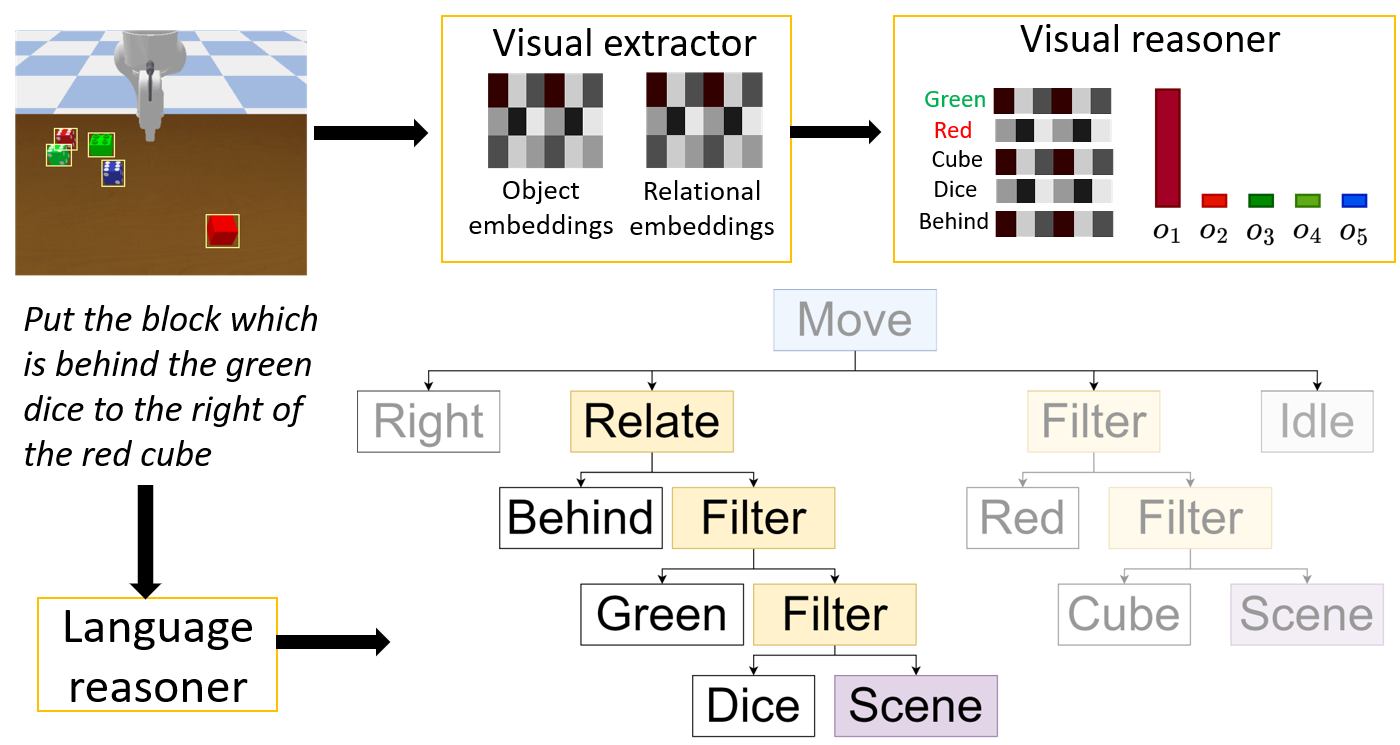
\includegraphics[width=\textwidth]{figures/example-1-n.png}
      \caption{Executing the emboldened sub-tree on the input scene}
      \label{fig:approach-1}
  \end{subfigure}

  \vspace{1cm}
  
  \begin{subfigure}{\textwidth}
      \centering
      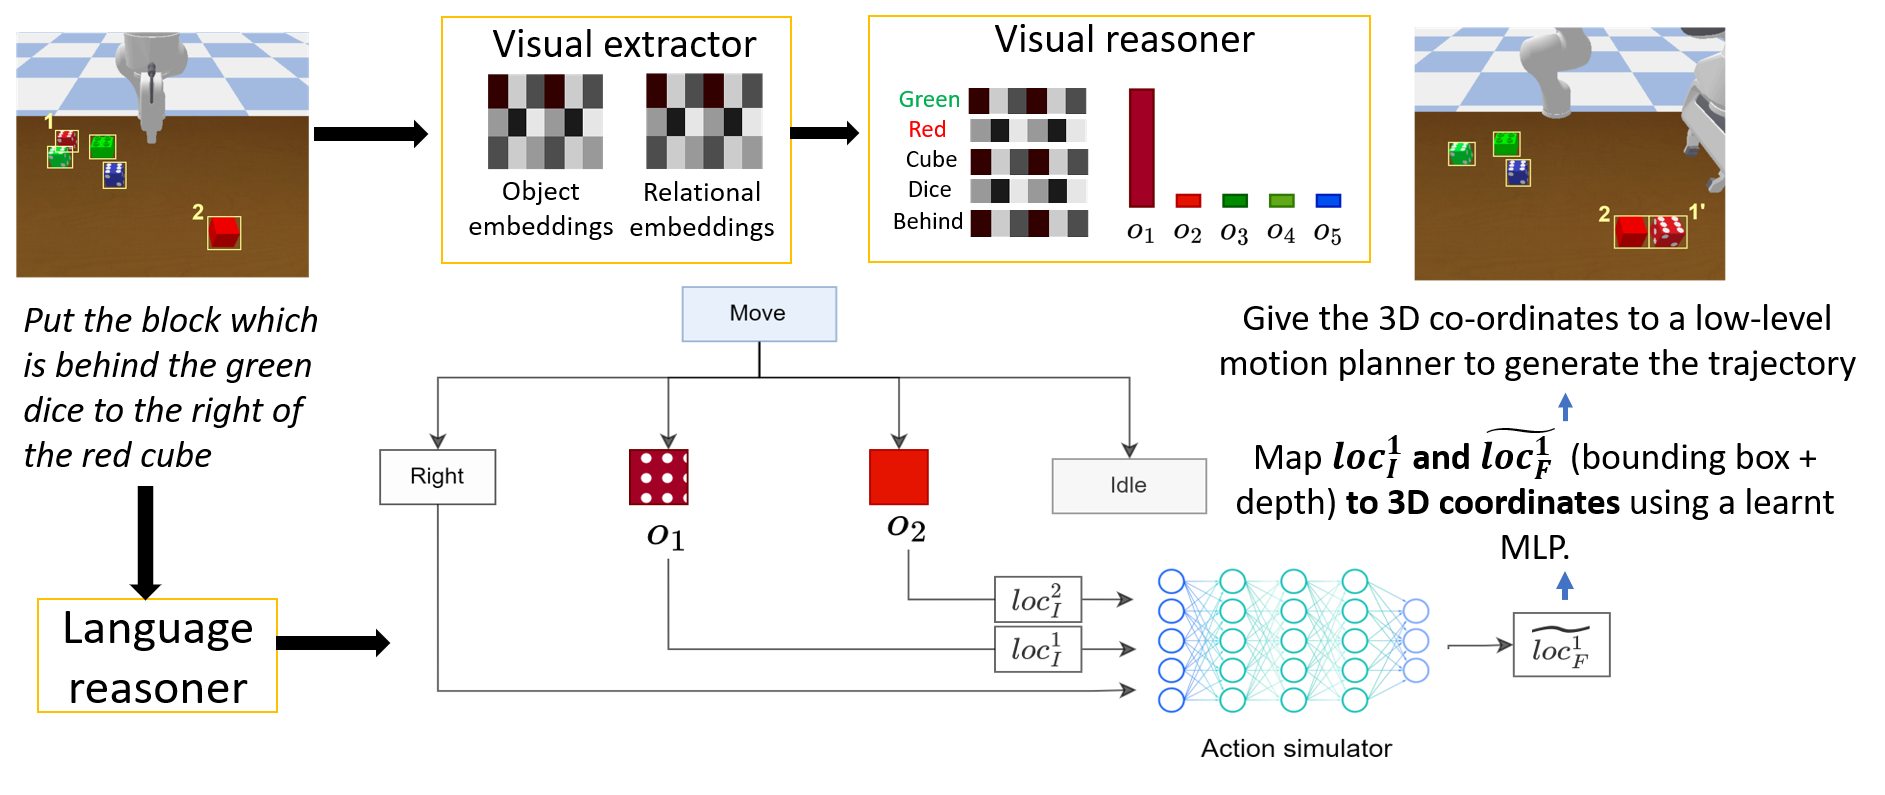
\includegraphics[width=\textwidth]{figures/example-2-n.png}
      \caption{VR computes the grounded program, which is used by the AS to compute the final location of the moved object, which is is fed into a low-level motion planner}
      \label{fig:approach-2}
  \end{subfigure}
  \caption{Quasi-symbolic program execution}
  \label{fig:approach}
\end{figure}

% Language Reasoner.
\subsection{Language Reasoner (LR)}
%
The language reasoner (LR) deduces a hierarchical symbolic program that corresponds to the 
manipulation task implied by the human's utterance to the robot. 
%
The deduced program consists of symbolic reasoning constructs that operate on neural concepts grounded in the state space of the scene and the action space of the robot. 
%
% Note that representation of a task as a hierarchical and compositional program facilitates deep reasoning over grounded concepts. 
%provided by symbolic constructs operating over grounded concepts. 
%
% Since a high-level task instruction may imply a sequence of actions, we adopt a hierarchical module where an LSTM~\cite{lstm} network first splits  the language instruction into a sequence of sub-instructions, each corresponding to one grounded action. The semantic parse of each sub-instruction is then inferred using a hierarchical  \emph{seq2tree} architecture similar to~\cite{dong2016language,Mao2019NeuroSymbolic}. The sequence of programs thus generated are composed to produce the symbolic program for the original language instruction.
% 
Since a high-level task instruction may imply a sequence of actions, we adopt a hierarchical model where an LSTM~\cite{lstm} network first splits the instruction into a sequence of sub-instructions, each corresponding to one grounded action. The semantic parse of each sub-instruction is then inferred using a hierarchical  \emph{seq2tree} architecture similar to~\cite{dong2016language,Mao2019NeuroSymbolic}. The sequence of programs thus generated are composed to produce the symbolic program for the original language instruction.
%
%
% Overall the LR module resembles a \emph{seq2tree} architecture that builds on ~\cite{dong2016language,Mao2019NeuroSymbolic} 
%
%The language reasoner (LR) has two parts (i) a splitter that breaks a multi-step instruction into a sequence of single step instructions, and (ii) a semantic parser, similar to ~\cite{dong2016language} and ~\cite{Mao2019NeuroSymbolic}, which takes each single step instruction and outputs a hierarchical program.  
%
%Formally, assuming a bound, $L_{max}$, on the word tokens representing a single step execution, 
%an arbitrary instruction $\Lambda = \lambda_{0:n} \coloneqq \{\lambda_0, \lambda_1,\cdots,\lambda_n\}$, at every step $t$, the splitter first decides a part of the sentence $\lambda_{0:l_t} \subset \lambda_{0:L_{max}}$ to be processed. The parser then takes $\lambda_{0:l_t}$ and  outputs a program $p_t$. The processed sub-string $\lambda_{0:l_t}$ gets removed and the process continues with the remaining part $\lambda_{l_{t}+1:n}$ of the instruction.
%Finally, the programs $p_1,\cdots p_T$ are composed into a single program $\mathtt{P}$, which will be used by the Visual Reasoner for grounding and execution. 


%For predicting the break point $l_t$, at the step $t$, the splitter encodes the first $L_{max}$ tokens it encounters using an LSTM [64] and outputs the hidden state, $h_t$ for each token. Then, a fully connected layer followed by a soft max layer outputs a probability distribution over the tokens for choosing a potential break point. The architecture of the semantic parser is very similar to that of the seq-to-tree parser (with slight changes in the kind of attention used) proposed by ~\cite{dong2016language} and later used by ~\cite{Mao2019NeuroSymbolic}; we refer to prior work for details.
%; we make use of additional attention with few extra attention to deal the action concepts. 

% VE Module
\subsection{Visual Extractor (VE)}
\label{subsec:visual-reason}
The visual extractor forms an object-centric view of the world by extracting object proposals in the form of bounding boxes for the objects using a pre-trained object detector~\cite{redmon2016you}. 
%
Following~\cite{Mao2019NeuroSymbolic}, dense object representations are obtained by passing the bounding boxes (after non-maximal suppression) through a feature extractor as~\cite{targ2016resnet}. 
The data association between object proposals in initial/final scenes is estimated greedily based on cosine similarity between the dense object features in both scenes.

% Visual Reasoner
\subsection{Visual Reasoner (VR)}
%
The visual reasoner performs visuo-spatial, object-centric reasoning to compute a sequence of sub-goals grounded in the scene from the symbolic program.
%
E.g., the instruction \textit{``put the block which is behind the green dice"} requires the robot to perform reasoning to resolve the specific world object that conforms to the relations/attributes as being behind a dice with colour attribute of green. 

The visual reasoner parameterizes object-level and relational concepts in the DSL (Table ~\ref{table:dsl}) with neural embeddings. Similar to ~\cite{Mao2019NeuroSymbolic}, a differentiable framework is defined for the execution of operators such as \emph{Filter, Unique, Relate, Idle}.  \\ 
%
As in ~\cite{Mao2019NeuroSymbolic}, intermediate results of execution are represented in a probabilistic manner. For e.g., a set of objects is represented as a vector of probabilities where the $i$-th element represents the probability of the $i$-th object being an element of the set. \emph{Filter, Unique, Relate} etc. sequentially modify this vector to ultimately yield the referred object/set of objects.  \\ 
%
This execution framework is used to execute the symbolic program  on top of the visual features (extracted by the visual extractor) resulting in the grounding of the program, $\Pi$, on the world state.


% Action simulator
\subsection{Action Simulator (AS)}
\label{subsec:action-simulator}
The action simulator learns the semantics of action concepts of the DSL. It takes as input, the action concept, the initial locations  of the object to be manipulated and the reference object respectively and outputs the target location of the former. The outputted target location of the object being manipulated serves as a sub-goal for the low-level motion planner. We determine the location of an object by the corners $b = (x_1,y_1,x_2,y_2)$ of the enclosing bounding box and the depth of the object from the camera face. 

\noindent  
Overall, the model can be summarized as follows:
\begin{itemize}
    \item $\mathtt{P} \leftarrow \mathtt{LR}(\Lambda; \theta_P, \theta_S)$, where $\mathtt{P}$ is a symbolic program composed of DSL constructs. 
    \item $\Pi \leftarrow \mathtt{VR}(\mathtt{P}, \mathtt{VE}(S_I;\theta_E);\theta_V)$. The visual reasoner then grounds $\texttt{P}$ and outputs $\Pi$, the grounded program. For example, in Figure \ref{fig:schematic}, red and blue subprograms are grounded to object 1 and 2 respectively.
    \item $G \leftarrow \text{AS}(\Pi; \theta_A)$. The action simulator then takes $\Pi$ and returns a sequence of sub-goals, $G = (g_0, g_1, ..., g_{n-1})$, for the motion planner.
\end{itemize}
Here, $\theta$'s are the parameters of the corresponding  module. 

\subsection{Loss Function and Model Training}
\label{subsec:loss&training}
%Model training optimizes the following loss:
%Let $\Theta$ = ($\theta_E$, $\theta_S$, $\theta_P$, $\theta_V$, $\theta_A$) be the parameters of the visual extractor, splitter, parser, visual reasoner and the action simulator respectively. Given instruction $\Lambda$ and initial scene $S_I$, 
% \\[-1cm]
% \begin{align*}
% \begin{split}
%      \mathtt{P} \leftarrow LR(\Lambda ; \theta_P, \theta_S) \\ 
%      \widetilde{S}_F & \leftarrow ManipulationProgram(S_I, \Lambda)\\[-0.1cm]
%      & \resizebox{0.9\hsize}{!}{ $=  AS\Big(VR\big( LR$(\Lambda ; \theta_P, \theta_S), VE(S_I ; \theta_E) ; \theta_V\big) ,LR(\Lambda ; \theta_P, \theta_S); \theta_A} \Big)\\
% \end{split}
% \end{align*}
% \\[-1cm]
%\begin{align*}
%    \resizebox{\hsize}{!}{\widehat{\Theta} \leftarrow \text{argmax}\limits_{\Theta} \;\mathbb{E}_\mathtt{P}\Big[\text{IoU}\big(S_F, Simulate(\mathtt{P} = ManiProg(S_I, \Lambda; \Theta))\big) \Big]}
%\end{align*}
%\textbf{Training on single-step instructions}. 
Given a single-step instruction $\Lambda$, the parser predicts a symbolic program $\mathtt{P}$. The visual reasoner grounds $\mathtt{P}$ to predict a sequence of sub-goals. The action simulator computes the low-level action corresponding to each sub-goal. The sequence of low-level actions is executed on the initial scene $S_I$ to get the predicted final locations of the objects $\{\widetilde{loc}^i_F\}_{i=1}^N$. Let $\{{loc}^i_F\}_{i=1}^N$ be the true locations in the gold final state, $S_F$. As mentioned above $loc = (b,d)$, where $b$ is the corners of bounding box and $d$ is the depth. The loss function $L_{act}\coloneqq \sum_i^N\|\widetilde{loc}^i_F- loc^i_F\|
+ \beta (1-\text{IoU}(\widetilde{b}^i_F, b^i_F))$ is used to train the action simulator and the visual modules. 
Since there is no explicit supervision to the parser, we train the parser using the policy gradient algorithm REINFORCE with the reward set to $-L_{act}$. 
%
During initial training, an explicit expectation (subtracting the mean action loss as the baseline) is computed over all programs to inform the loss, ameliorating the variance issue arising in REINFORCE.
%
The Language Reasoner is trained using REINFORCE and the other modules using backpropagation.
%
%expectation over $\mathbb{E}_{\mathcal{P}}[-L_{act}(P)]$ over the program space $\mathcal{P}$ and use this as reward to the parser.
%
 %The parameters $\theta_E$, $\theta_V$ and $\theta_A$ are trained by back propagation from the expected action loss, $\mathbb{E}_{\mathcal{P}}[L_{act}(\mathtt{P})]$, and $\theta_P$ is trained by REINFORCE using $\mathbb{E}_{\mathcal{P}}\big[\sum_{\mathtt{P}\in \mathcal{P}}{L_{act}(\mathtt{P})} + L_{par}(\mathtt{P})\big$]. 
%
\iffalse
Once we have trained the other modules on single step commands, we train the splitter on all one and two step commands in the training set. The splitter computes the probability $\mathcal{S}(s;\theta_s)$ of breaking the sentence on each token $s$ of the first $L_{max}$ tokens. The training objective, for a sentence $\Lambda$, can be described as 
\[
    \resizebox{\hsize}{!}{\[\theta_S \leftarrow \text{argmin} \Big( \mathbb{E}_{s\sim{\mathcal{S}}}\big[L_{act}(Compose(Parser(L_{0:s}),Parser(L_{s+1:}))\big]\Big)\]}
\]
 where $Compose$ takes input symbolic programs generated by the parser for single step instructions and composes them hierarchically. Since all other modules are already trained for single step sentences. The splitter learns to split the large sentences at the correct positions. 
 \fi
% We do not have direct access to the true plan $G$. We also do not have access to intermediate object locations. The only information we have is the locations of the objects in the  the final scene $S_F$.   Let $loc_i \equiv (b_i, d_i)$ denote the true location (in the image space) of object $i$, in the final scene $S_{T+1}$. Recall that $b_i, d_i$ are bounding box and mean depth of the object $i$ respectively. Let $\widehat{loc}_i$ denote the final location of object $i$ as predicted by our model. Then, we compute the loss (for object $i$) $\mathcal{L}(\widehat{loc_i},loc_i)$ as a combination of two terms, $w_1 * {\tt MSE}(\widehat{loc_i},  loc_i) +w_2 * (1- {\tt IoU}(\widehat{b_i}, b_i))$. The first term is the mean squared error between true and predicted locations, and the second term is one minus intersubsection over union (IoU) between the true and predicted bounding boxes. $w_1,w_2$ are hyper-parameters determining the important of two loss terms, and are set using a validation set. The total loss, $L$, is simply average of the loss over each object, i.e., $\sum_{i=1}^{N} \mathcal{L}(\widehat{loc_i}, loc_i)/N$. The reward signal passed to the parser is computed as, $R  = R_0 - L$ where $R_0$ is a hyper-parameter.

The following training curriculum is adopted: (i) training on single step commands with reasoning involving individual object features only, 
(ii) the trained action simulator module is frozen and additional training on single step commands involving reasoning over spatial relations between objects is carried out. 
(iii) the sentence splitter in the Language Reasoner module is fine-tuned on multiple-step instructions. 

\subsection{Scene Reconstruction}
We additionally train a neural model to synthesize the scene corresponding to each sub-goal, given only the initial scene and predicted object locations. This enables us to visualise the scene modification without the need of execution by a robot manipulator along with providing interpretability to the model's latent program space. Our approach is adapted from \cite{dhamo2020_SIMSG}.

\begin{figure}
    \centering
    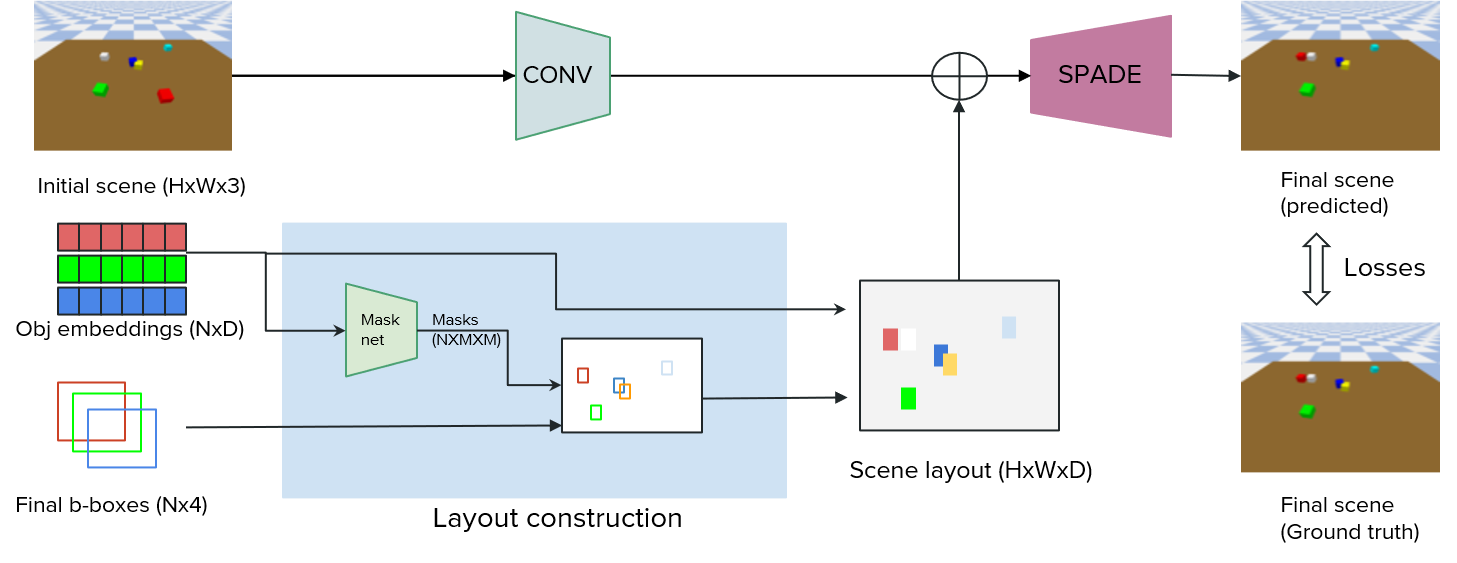
\includegraphics[width=\textwidth]{assets/recons-arch.png}
    \caption{Scene reconstruction architecture}
    \label{fig:recons}
\end{figure}

The reconstruction architecture can be seen in figure \ref{fig:recons}. The scene graph is constructed with nodes having object embeddings (N objects, each with an embedding of size D) and bounding boxes (N objects, each with a bounding box of size 4). This graph is updated with predicted bounding boxes corresponding to final locations of the objects after any given step. A scene layout is created by stacking the object features according to their corresponding final locations. This layout is concatenated with the initial image features, and passed through the SPADE decoder. The final scene is used for supervison, with a weighted sum of the several pixelwise and discriminator-based losses, similar to \cite{dhamo2020_SIMSG}. This trained model can now be used to reconstruct any intermediate scene, by updating the predicted bounding boxes in the scene graph corresponding to the subgoals at each step, as shown in figure \ref{fig:recons-steps}

\begin{figure}
    \centering
    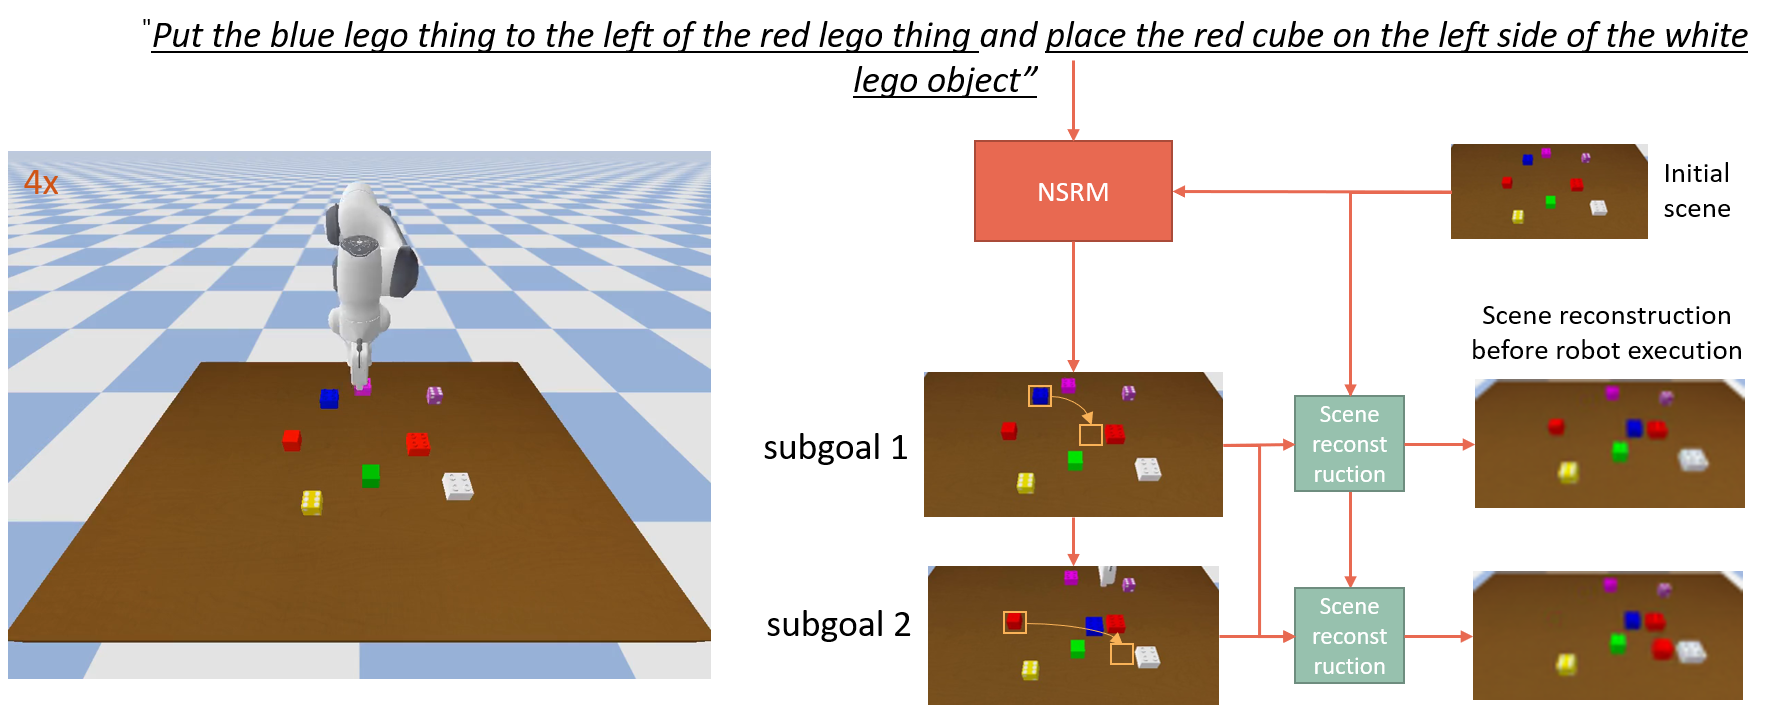
\includegraphics[width=\textwidth]{assets/recons-steps.png}
    \caption{Scene reconstruction at each step before the actual execution}
    \label{fig:recons-steps}
\end{figure}


\label{sec:evaluation}
%
% ~\textcolor{red}{q. this para can be removed for shortening perhaps}In our experiments we study (i) whether our method can infer 
% programs to translate instructions to desired goal states, 
% (ii) the extent to which the method generalizes to novel 
% instructions and world states and (iii) whether the model 
% can generalize to multiple step plans having been trained on 
% simpler plans and (iv) whether model predictions can be used by a simulated 
% robot to execute a task as well as hypothesize future world states. 

% Main accuracy results
\begin{table*}[ht]
    \centering
    \caption{Comparison between Proposed Model and NMN+ based on number of steps (BB: Bounding Boxes)}
    \begin{tabular}{|c|c|c|c|c|c|c|c|}
    \hline
         Model  & \multicolumn{3}{|c|}{Overall} &  \multicolumn{2}{|c|}{Single-step} & \multicolumn{2}{|c|}{Double step} \\ 
         \hline
         \hline
          & IOU & IOU-M & Program & IOU & IOU-M  & IOU & IOU-M \\
           &  &  & (Action/Subj/Pred) & &   &  &  \\
          \hline
         NMN+ (gold BB) & 0.77 & 0.55 & --/0.81/0.76 & 0.80 & 0.56 &    0.71 & 0.52 \\ 
         \hline 
         Ours (gold BB)  & 0.87 & 0.72& 0.99/0.99/0.94 & 0.91 & 0.64 &   0.87 & 0.62 \\
        \hline 
         NMN+ (extracted BB) & 0.69 & 0.32& --/0.81/0.55 & 0.78 & 0.49 &  0.58 & 0.22 \\ 
         \hline 
         Ours (extracted BB) & 0.76  & 0.41  & 0.99/0.74/0.76 &0.80 & 0.43  & 0.69 & 0.54 \\
         \hline 
    \end{tabular}
    % \vspace{1em}
    \label{tab:accuracy}
\end{table*} 

\begin{table*}[ht]
    \centering
    \caption{Comparison between Proposed Model and NMN+ based on instruction complexity  (BB: Bounding Boxes)}
    \begin{tabular}{|c|c|c|c|c|}
    \hline
         Model  & \multicolumn{2}{|c|}{Simple} & \multicolumn{2}{|c|}{Complex} \\ 
         \hline
         \hline
          & IOU & IOU-M & IOU & IOU-M  \\
            &  &  &  &   \\
          \hline
         NMN+ (gold BB) & 0.90 & 0.71 & 0.64 & 0.31\\ 
         \hline 
         Ours (gold BB)  & 0.92 & 0.73 & 0.87 & 0.64 \\
        \hline 
         NMN+ (extracted BB) & 0.79 & 0.55 & 0.60 & 0.20\\ 
         \hline 
         Ours (extracted BB) & 0.83 & 0.62 & 0.69 & 0.24\\
         \hline 
    \end{tabular}
    % \vspace{1em}
    \label{tab:accuracy2}
\end{table*} 


%%%%%%%%%%%%%%%%%%%%%%%%%%%
%%% EXPERIMENTAL SETUP %%%
%%%%%%%%%%%%%%%%%%%%%%%%%%%

% \begin{table*}[ht]
%     \centering
%     \caption{Accuracy Comparison for the Proposed Model and the Baseline}
%     \begin{tabular}{|c|c|c|c|c|c|c|c|c|c|c|c|c|c|c|c|c|}
%     \hline
%          Model  & \multicolumn{3}{|c|}{Overall} &  \multicolumn{3}{|c|}{Single-step} & \multicolumn{3}{|c|}{Double step} & \multicolumn{3}{|c|}{Simple} & \multicolumn{3}{|c|}{Complex} \\ 
%          \hline
%          \hline
%           & IOU & IOU-M & & Program & IOU & IOU-M & Program &  IOU & IOU-M & Program & IOU & IOU-M & Program & IOU & IOU-M  & Program \\
%           \hline
%          Baseline & 0.77 & 0.55 & 0.80 & 0.56 & 0.71 & 0.52 & 0.90 & 0.71 & 0.64 & 0.31\\ 
%          \hline 
%          Ours  & 0.87 & 0.72 & 0.91 & 0.64 & 0.87 & 0.62 & 0.92 & 0.73 & 0.87 & 0.64 \\
%         \hline 
%          Baseline + Perception & 0.69 & 0.32 & 0.78 & 0.49 & 0.58 & 0.22 & 0.79 & 0.55 & 0.60 & 0.20\\ 
%          \hline 
%          Ours + Perception & 0.76  & 0.41  & 0.80 & 0.43 & 0.69 & 0.54 & 0.83 & 0.62 & 0.69 & 0.24\\
%          \hline 
%     \end{tabular}
%     % \vspace{1em}
%     \label{tab:accuracy}
% \end{table*} 



% \begin{table}
%     \centering
%     \caption{Comparison of Proposed Model and CLIPort}
%     \begin{tabular}{|c|c|c|}
%          \hline 
%          Model  & Identification Accuracy & Placement Accuracy \\ 
%          \hline
%           CLIPort & 0.46 &  0.39  \\
%           \hline
%          CLIPort(x5) &  & \\ 
%          \hline 
%          Ours    & 0.94 & 0.93 \\
%         \hline 
%     \end{tabular}
%     % \vspace{1em}
%     \label{tab:cliport}
% \end{table} 


\begin{table}[ht]
    \large
    \centering
    \caption{Comparison b/w Proposed Model and CLIPort}
    \resizebox{\columnwidth}{!}{%   
    \begin{tabular}{|c|c|c|c|c|c|c|c|c|c|c|c|c|}
    \hline
         Model  & \multicolumn{2}{|c|}{Overall}  & \multicolumn{2}{|c|}{Simple} & \multicolumn{2}{|c|}{Complex} \\ 
         \hline
         \hline
          & Id. Acc. & Pl. Acc. & Id. Acc.  & Pl. Acc. & Id. Acc.  & Pl. Acc.   \\
          
          \hline
            CLIPort & 0.46 & 0.39 & 0.55 & 0.47 & 0.32 &    0.26 \\ 
         \hline 
                     CLIPort(5x) & 0.76 & 0.61 & 0.90 & 0.74 & 0.55 &    0.39 \\ 
                     \hline 
         Ours (gold BB)  & 0.94 & 0.93 & 1.0 & 1.0  & 0.83 & 0.81  \\
         \hline 
    \end{tabular}%
    }
    % \vspace{-0.25in}
    \label{tab:cliport}
\end{table} 





\subsection{Experimental Setup}
%%% DATA %%%
\textbf{Data collection. } 
The dataset is collected in a PyBullet tabletop environment using a 
simulated Franka Emika Panda robot arm. The workspace consists of a tabletop with blocks of different shapes and colors.
%
Each datapoint consists of an initial scene paired with a language instruction and the expected resulting final scene. We provide a framework for quickly simulating and generating data for an arbitrary length instruction on a scene with any number of objects.
For training, close to 5000 synthetic scenes and language instructions(with a 80:20 train-test split) are sampled with 3-5 blocks of varying colors and shapes and placed at randomized orientations on the table. 
%
% The instructions range from single physical pick-place operation \emph{``Put the red block on the green block"} to ones involving a composition of such operations like \emph{``Put the red block which is behind the white dice to right of the blue cube, then put the lego block on top of red block"}. 
%
%The robot's motion skills are realized using a crane grasping for
%picking and re-positioning the object at the target pose.

The dataset consists of both single-step(e.g. \emph{``Put the red block on the green block"}) and double step commands(e.g. \emph{``Put the red block which is behind the white dice to right of the blue cube, then put the lego block on top of red block"}). 
On the basis of the level of reasoning involved in the given instruction, we can classify the dataset into (i) \textit{simple} that involve reasoning over individual object features only and \textit{complex} that additionally involve reasoning over inter-object relationships.

%%% BASELINE %%%
\subsection{Baselines, Metrics and Comparisons} 
The proposed model (i) performs visuo-linguistic reasoning in a symbolic latent space and (ii) assumes an object-centric state representation. We provide comparisons with baselines that forego these two assumptions.

% \textbf{CLIPort}~\cite{shridhar2022cliport} performs language-guided manipulation by leveraging the visual and linguistic semantics embedded in pre-trained CLIP~\cite{clip}. Unlike ours, the model lacks explicit, modular constructs to perform the reasoning inherent in object manipulation tasks.} ~\textcolor{red}{TODO: Add explanation for table3 

\textbf{NMN+}, inspired from Neural Module Networks \cite{andreas2016neural}, assumes an object-centric state representation. However, in contrast to the proposed model, visuo-linguistic reasoning required for manipulation is performed using language-guided attention over object embeddings instead of using symbolic reasoning constructs. %Figure~\ref{fig:nmn} provides the detailed architecture. 
The entire architecture is neural and is trained end-to-end with the loss same as that of the proposed model. 

% For a fair evaluation, our model and the baseline share the instruction encoder, the action simulator and the object feature extractor. The baseline includes an action decoder and four attention modules divided into two groups of two each. Each group takes in the encoded instruction and embedding for all objects present in scene and predicts two objects involved in manipulation. The location of the predicted objects and output of the action decoder is the input to the action decoder, that provides the predicted location as output. Here, \textit{location} includes both the bounding box and depth of the object. 



% \begin{figure}
% \begin{subfigure}{1.0\hsize}
%      \centering    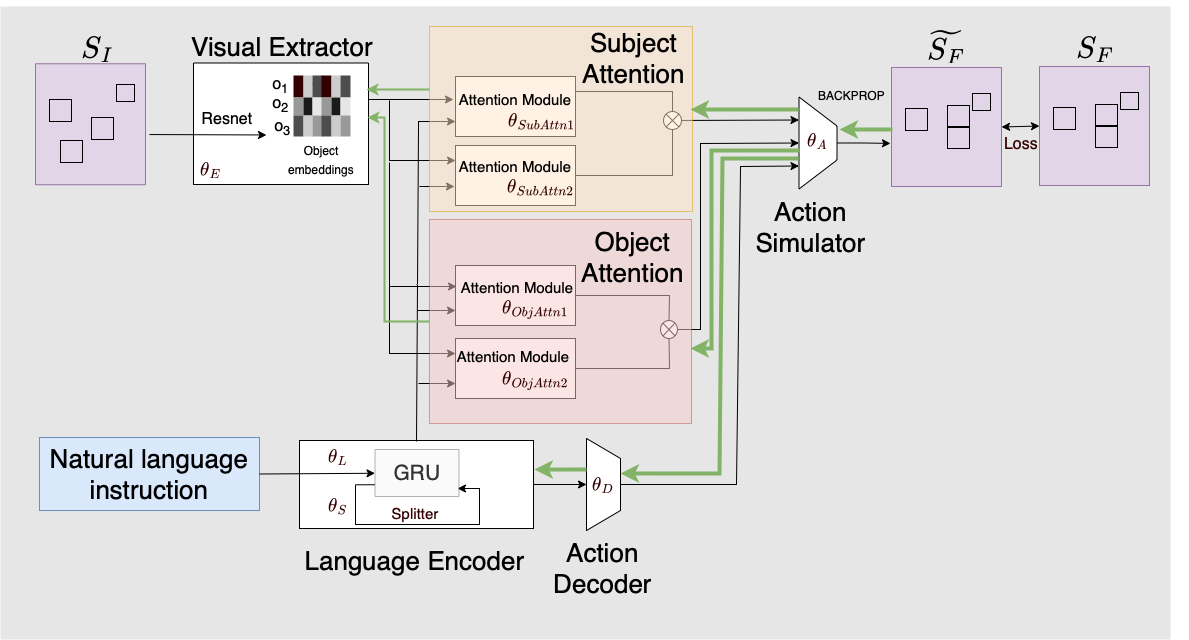
\includegraphics[width=\textwidth]{figures/baseline.png}
% \end{subfigure}
% \caption{
%     \footnotesize{
%         \textbf{Object-centric baseline NMN+.} For a fair comparison, our model and NMN+ share the same language encoder (with LSTM-based splitter) and the visual extractor. Attention blocks compute language-guided attention over object embeddings to get the \emph{subject} and \emph{predicate} for the manipulation action. This is fed into the action simulator along with the action embedding from the action decoder to get the predicted final location of the object.}}
%         \vspace{-0.15in}
%             \label{fig:nmn}
% \end{figure}

The following metrics are used for comparing the proposed model with \emph{NMN+}:
\begin{enumerate}
    \item \emph{Intersubsection over Union (IOU)} of the predicted and groundtruth bounding box is calculated in the 2D image space assuming a static camera viewing the scene. Average IOU over all objects in the scene and mean IOU for objects moved during execution, termed IOU-M,  are reported.
    \item \emph{Program Accuracy}: The grounded program inferred for an (instruction, scene)-pair using the proposed model is compared with the manually annotated ground truth program. We separately report the grounding accuracy for the subject and predicate of our action (assumed binary) and the accuracy of the predicted action inferred from the instruction. Since, there is no explicit notion of grounded actions in the baseline, we do not report this metric for the baseline. 
\end{enumerate}    

\begin{figure}[h!]
\begin{subfigure}{0.5\hsize}
     \centering    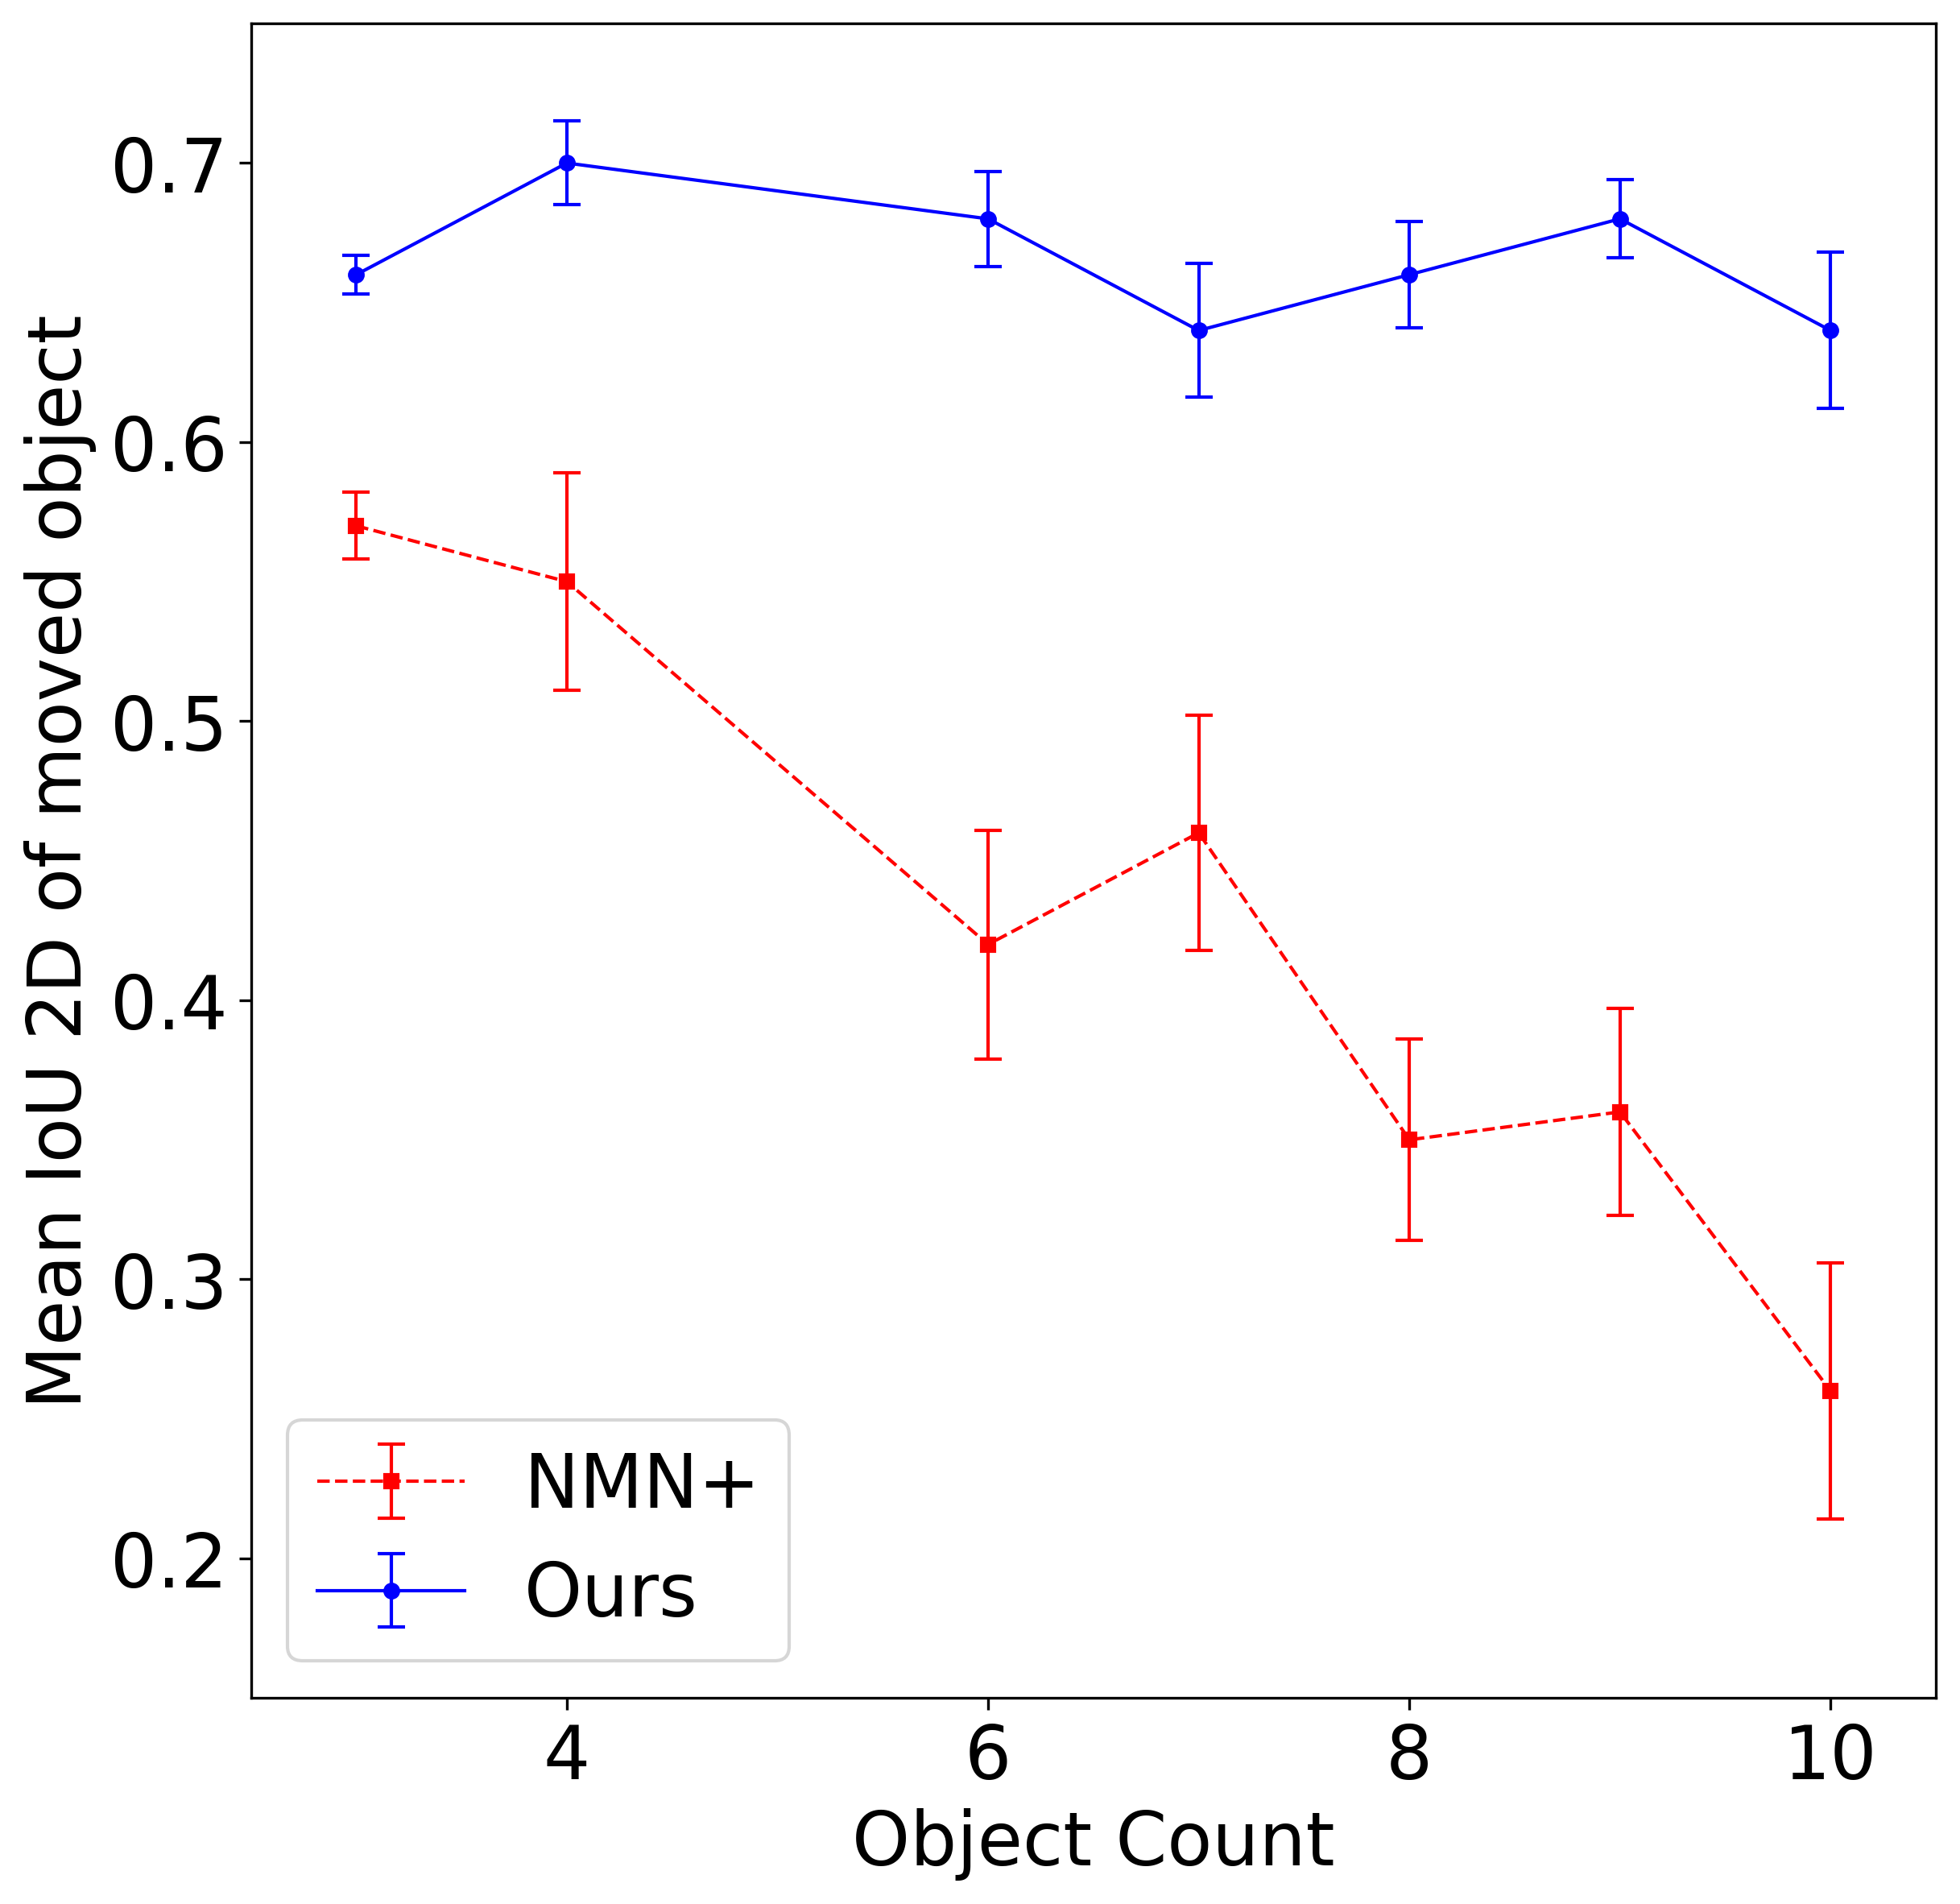
\includegraphics[width=0.8\textwidth]{figures/multi-object-1.png}
    \caption{\footnotesize{IoU vs \# of objects}}
    % IoU of the predicted position of the object moved during execution with its ground truth position v/s number of objects in the scene.
    \label{fig:large_scenes}
\end{subfigure}%
% Generalization on larger steps
% \begin{figure}[!h]
%     \centering
%     \subfigure{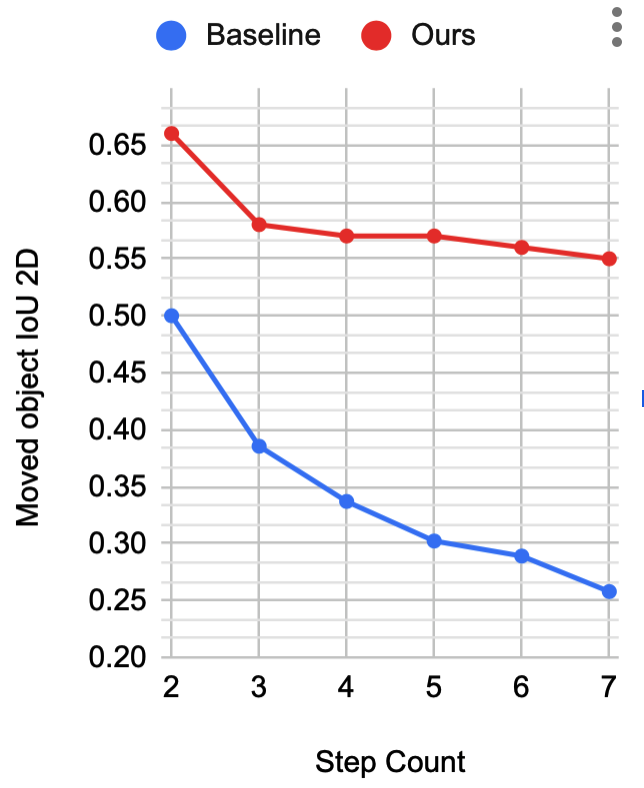
\includegraphics[width=0.2\textwidth]{figures/large_steps.png}} 
%     \subfigure{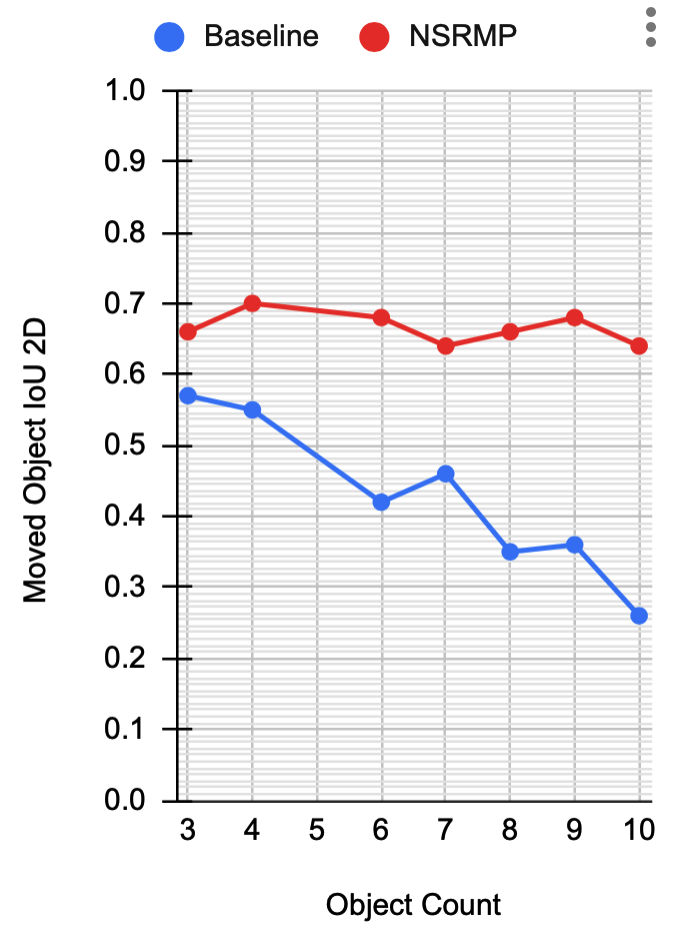
\includegraphics[width=0.2\textwidth]{figures/generalization_large_scenes.png}} 
%     \caption{Caption}
%     % \label{fig:foobar}
% \end{figure}
\begin{subfigure}{0.5\hsize}
     \centering    
     %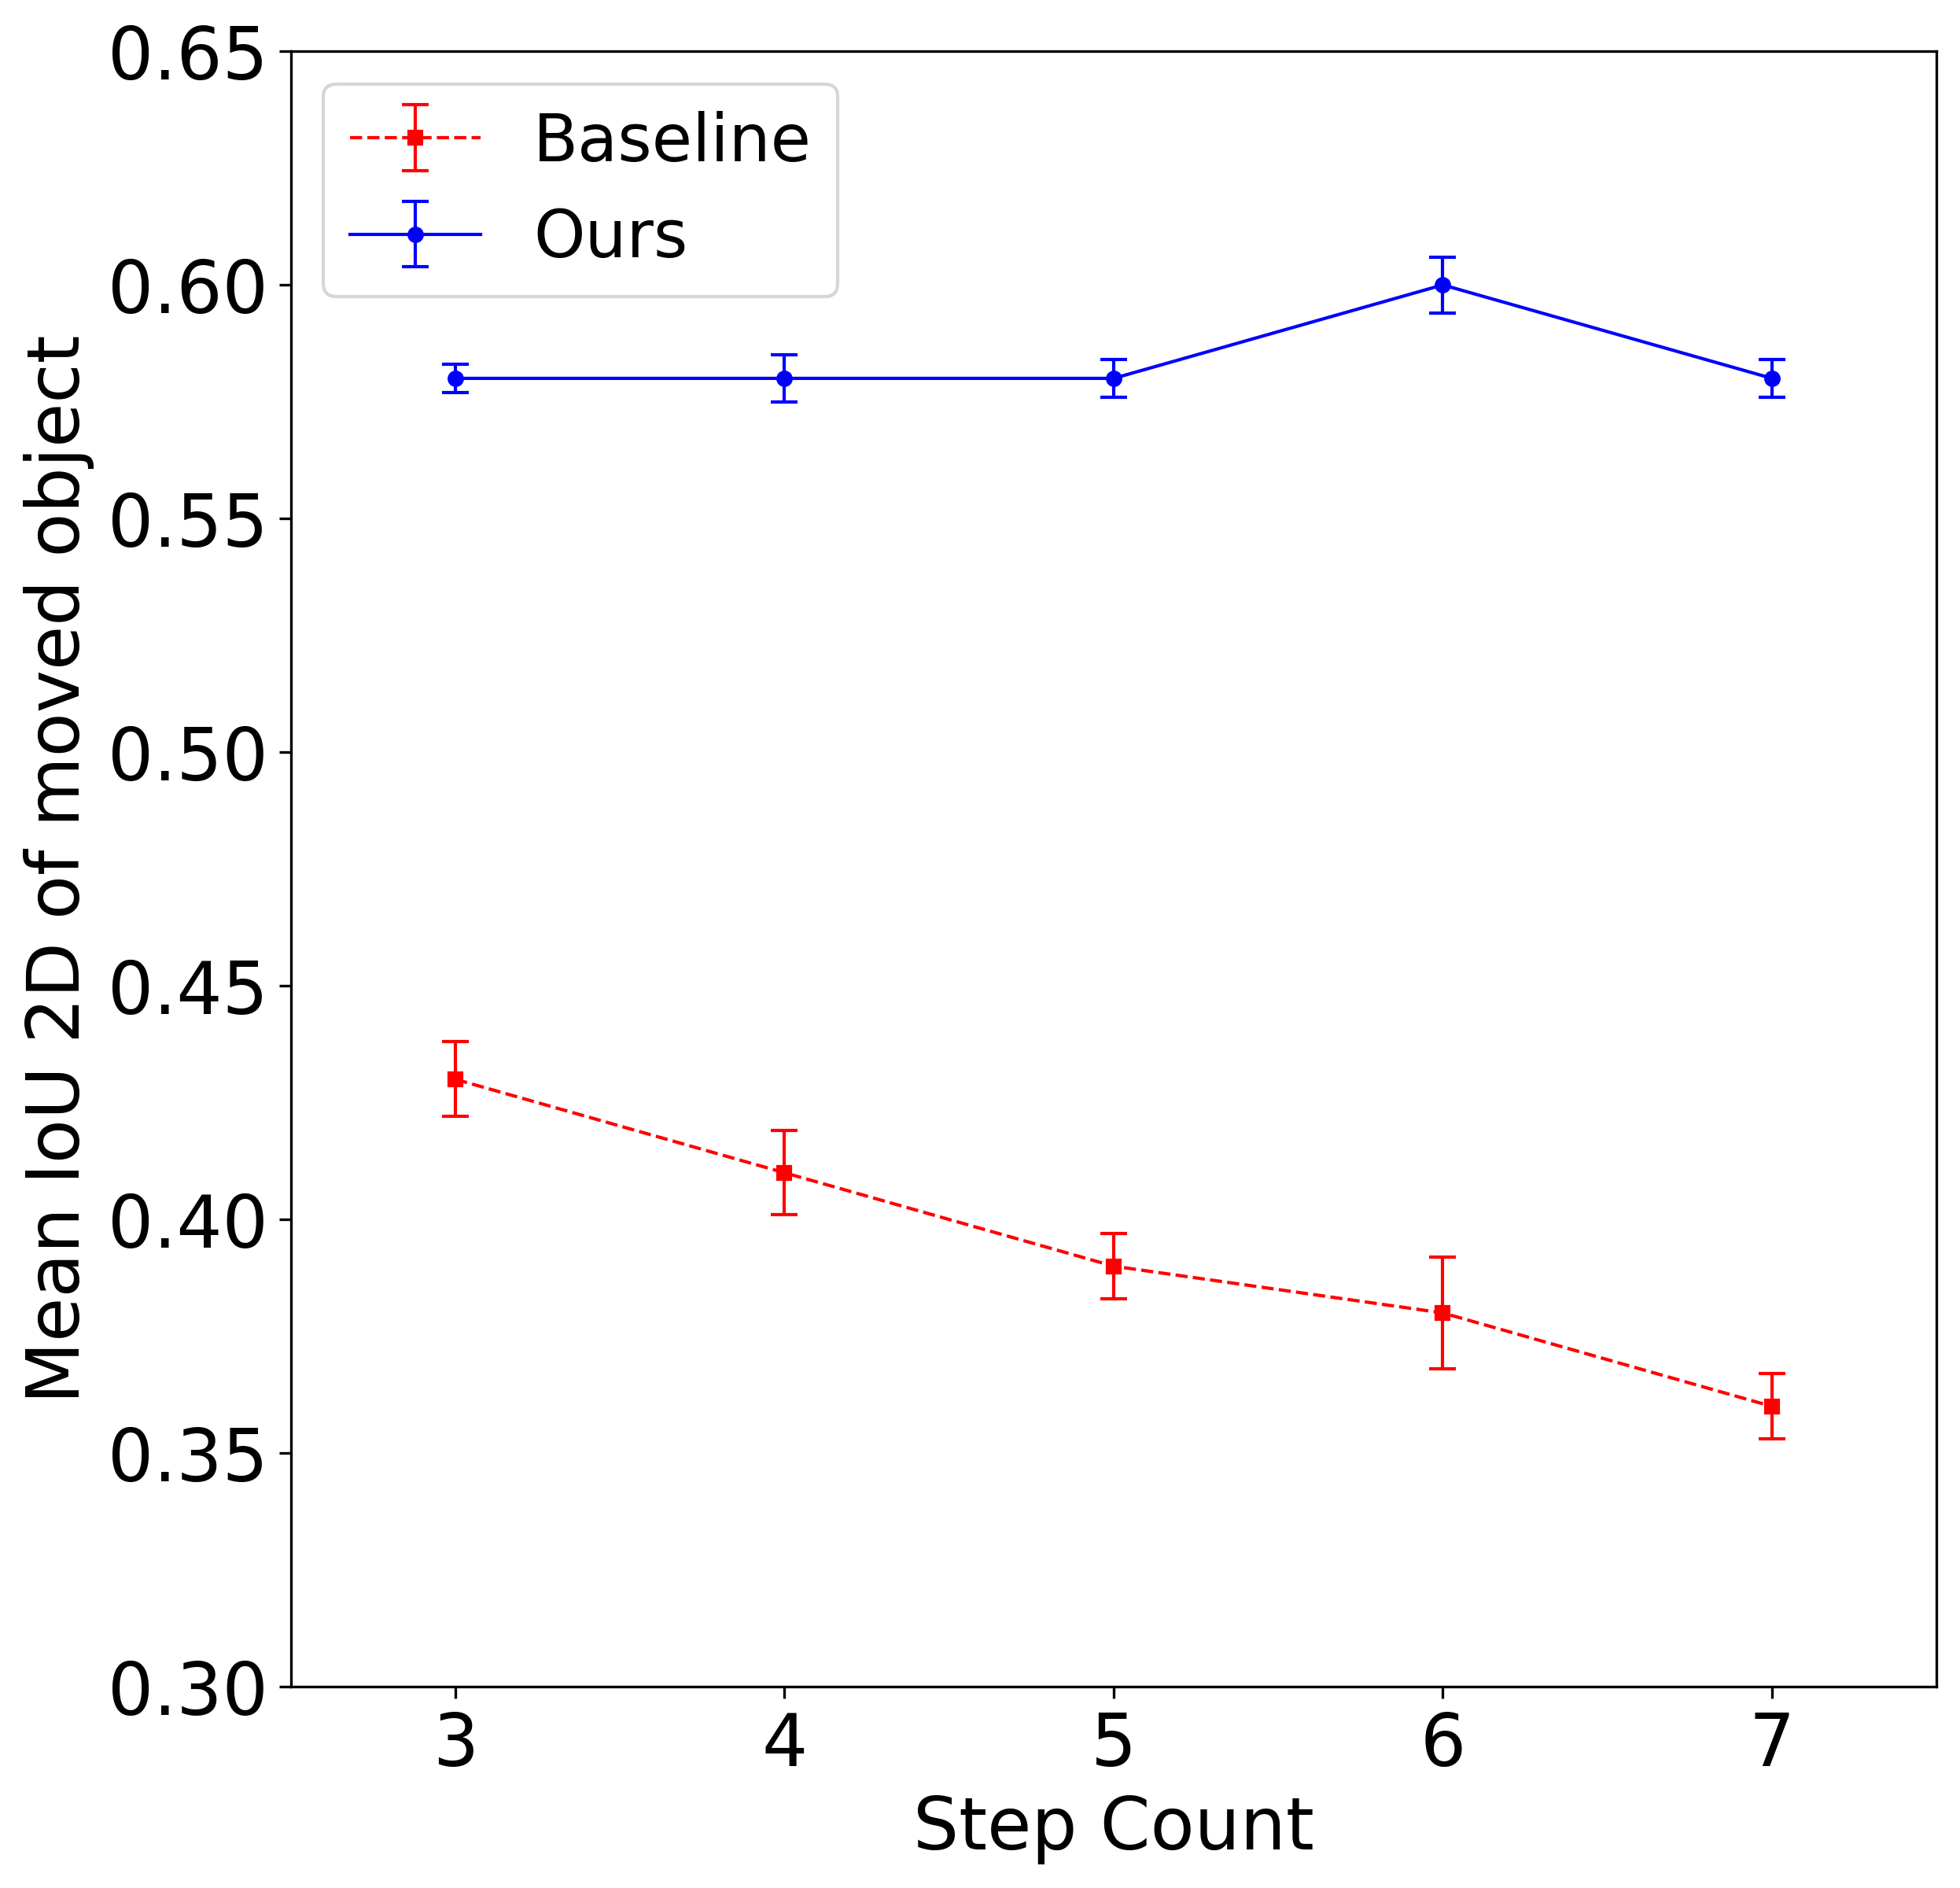
\includegraphics[height=4.375cm,width=3cm]{figures/multi-step.png}
     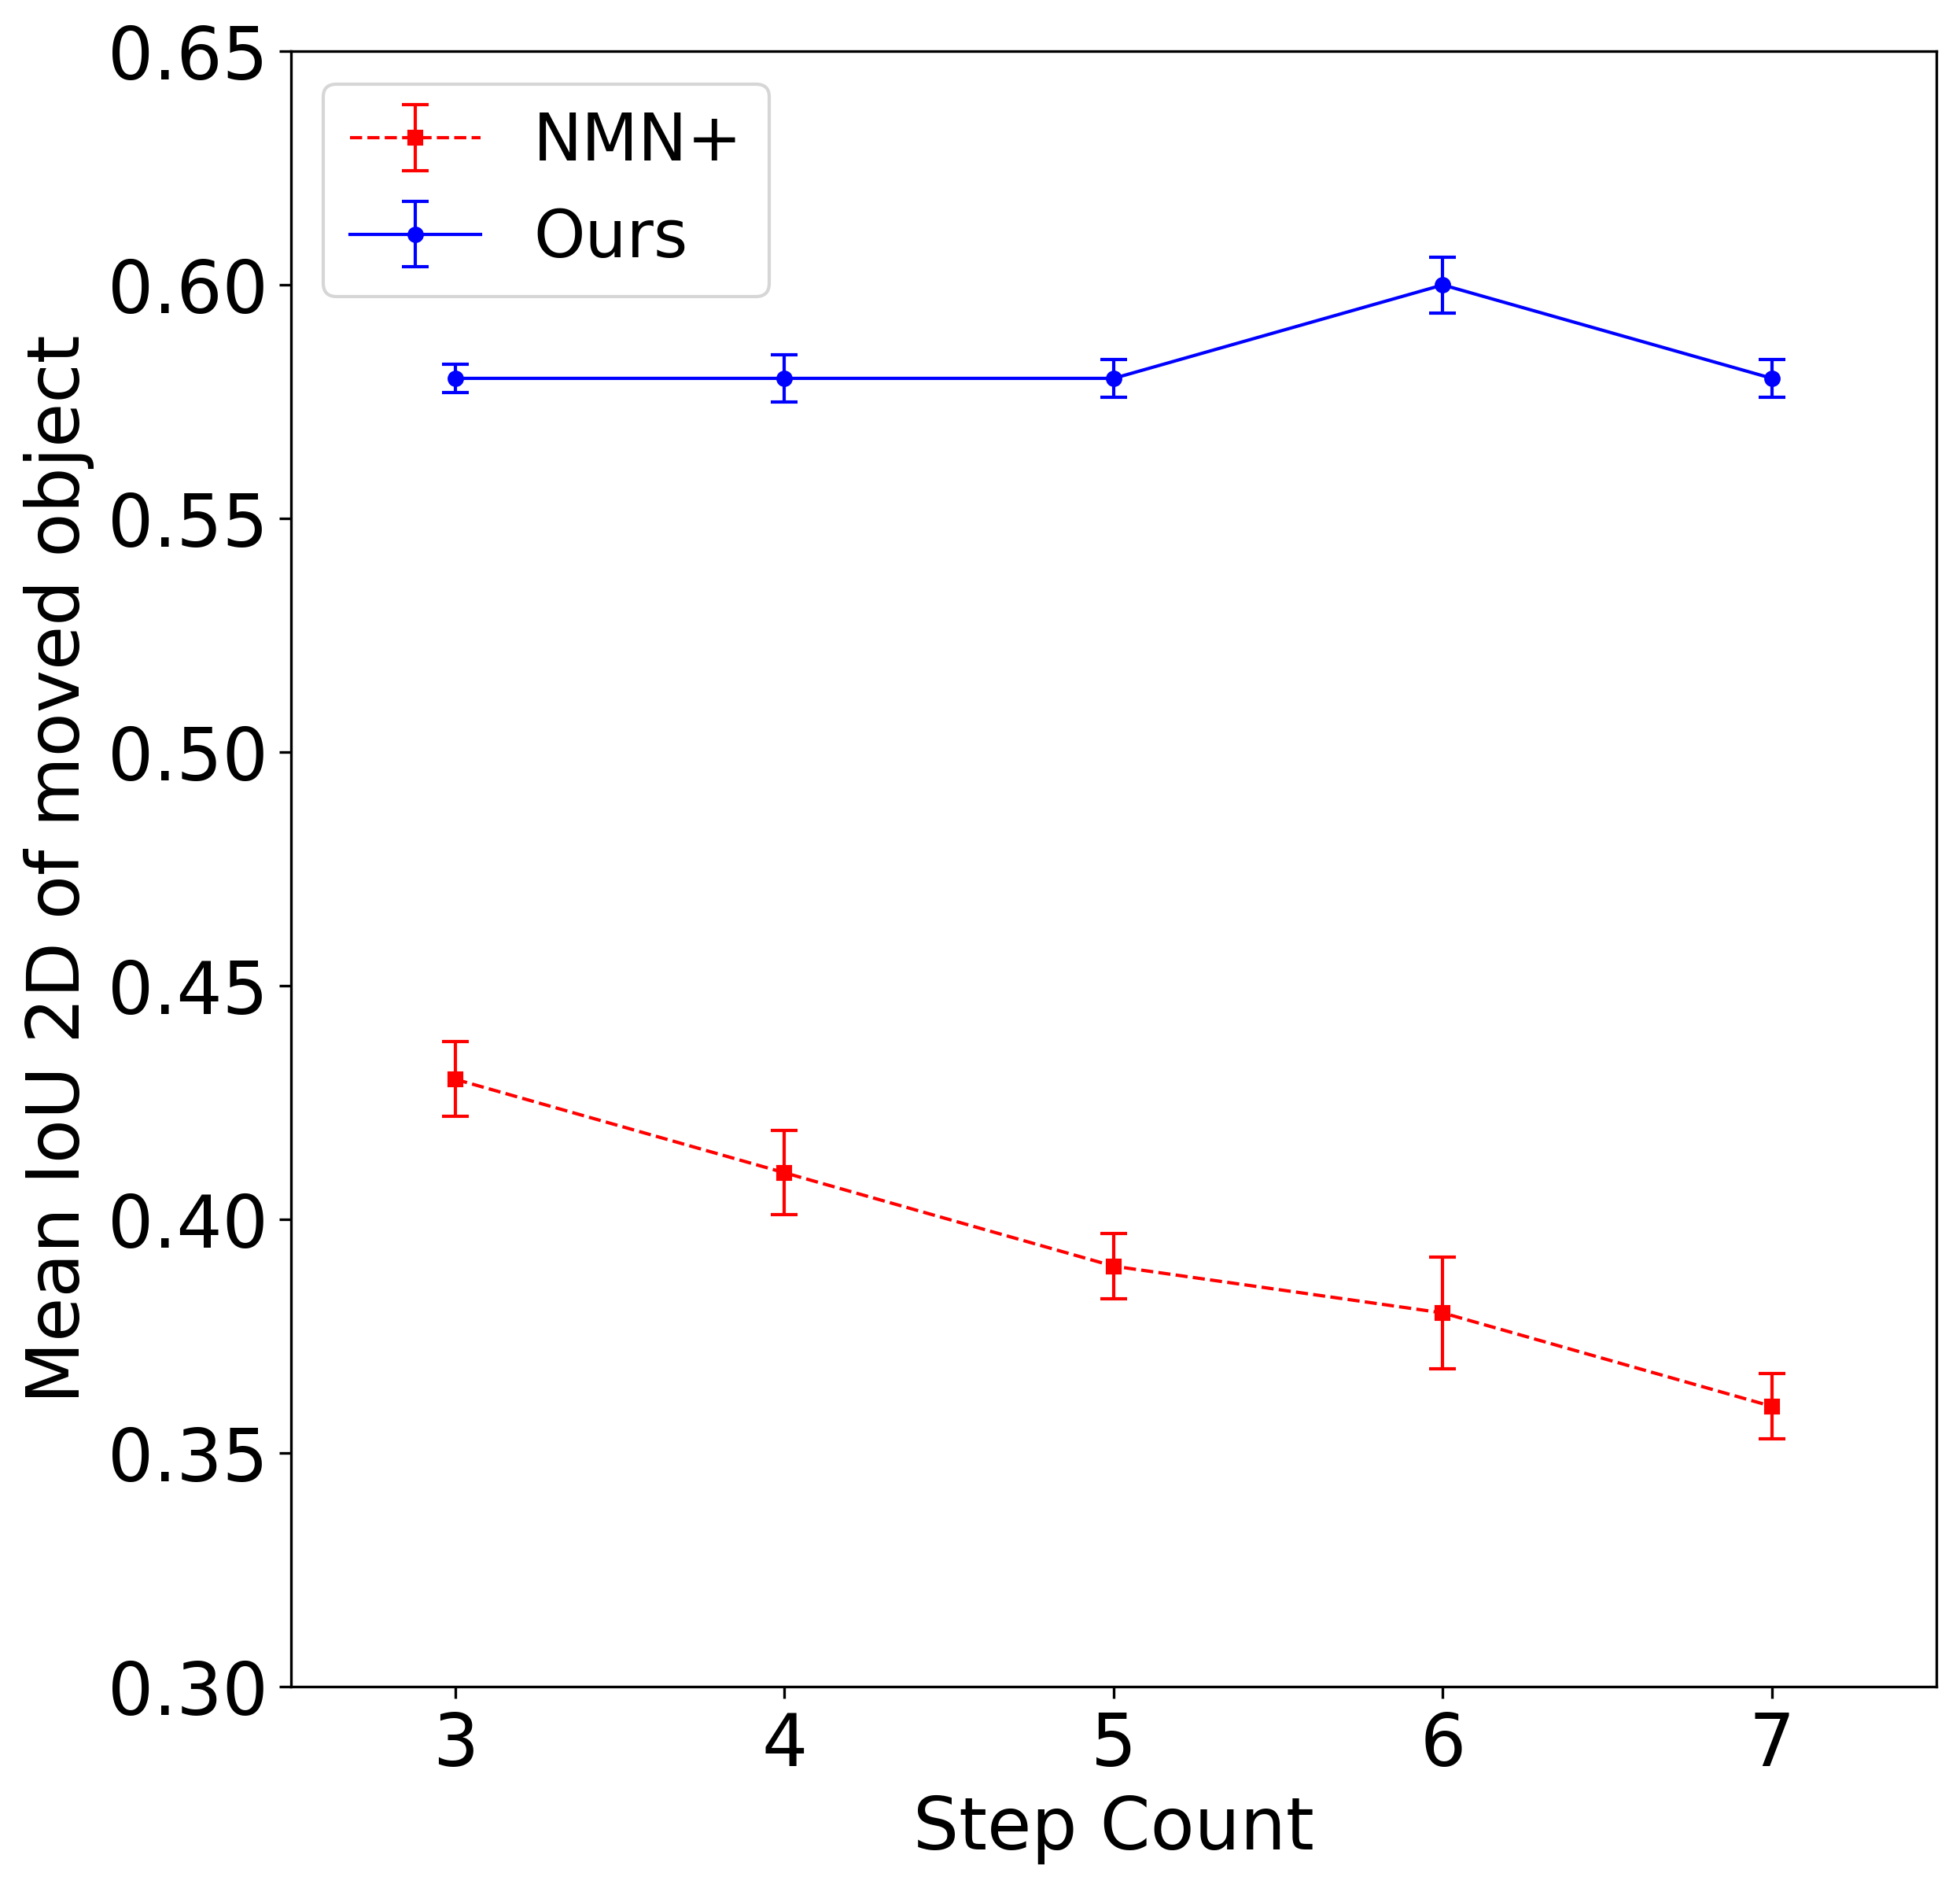
\includegraphics[width=0.8\textwidth]{figures/multi-step-1.png}
    \caption{\footnotesize{IoU vs varying \# of steps}}
     %IoU of the predicted position of the object moved during execution with its ground truth position v/s number of atomic actions implied in the instruction.
    \label{fig:large_steps}
\end{subfigure}
\caption{\footnotesize{Performance in generalization settings}}
% \vspace{-0.15 in}
\end{figure}


% \begin{figure*}[hbt!]
%     \centering    
%     \includegraphics[width=16.5cm]{figures/row2a.png}
%     \label{fig:qual-1}
% \end{figure*}
% \begin{figure*}[hbt!]
%     \centering    
%     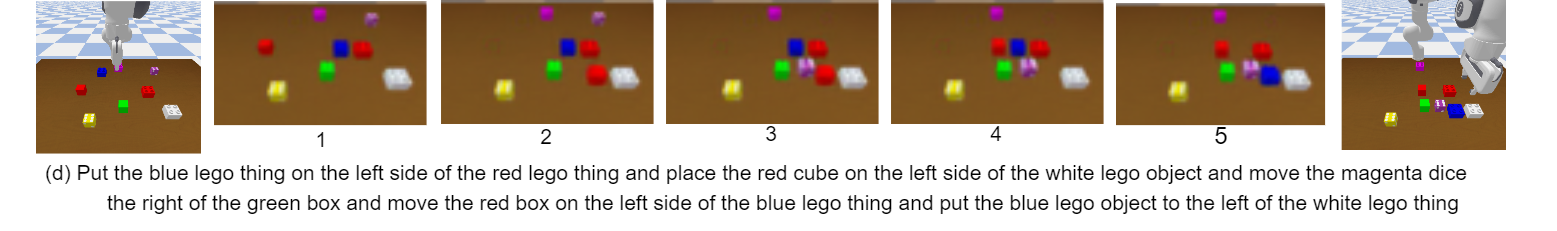
\includegraphics[width=17cm]{figures/row2b.png}
%     \caption{
%     \footnotesize{
%     Execution of robot manipulator on (a) compound instructions, (b) scene with 15 objects, (c) double step instruction with relational attributes, (d) 5-step instruction. (d) also shows reconstruction of the predicted scene before each step of the simulation
%     }}
%     \label{fig:qual-1}
%     % \vspace{-0.1 in}
% \end{figure*}

\begin{figure}
    \centering
    \hfill
    \begin{subfigure}{0.45\textwidth}
        \centering
        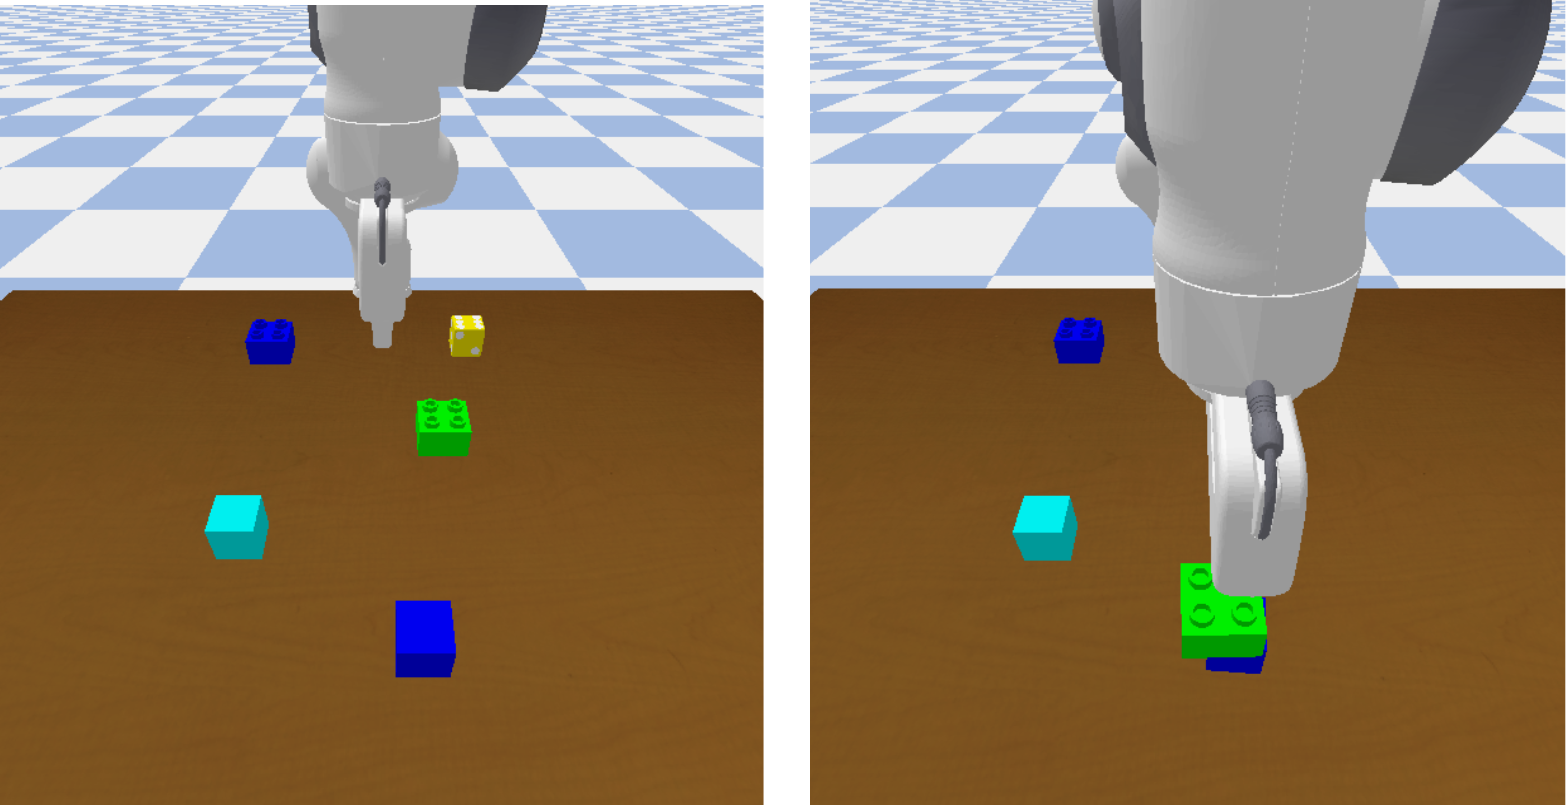
\includegraphics[width=\textwidth]{assets/qual-1.png}
        \caption{A compound instruction, \footnotesize{"Move the block which is a lego and green in color on top of the cube whose color is blue"}}
    \end{subfigure}
    \hfill
    \begin{subfigure}{0.45\textwidth}
        \centering
        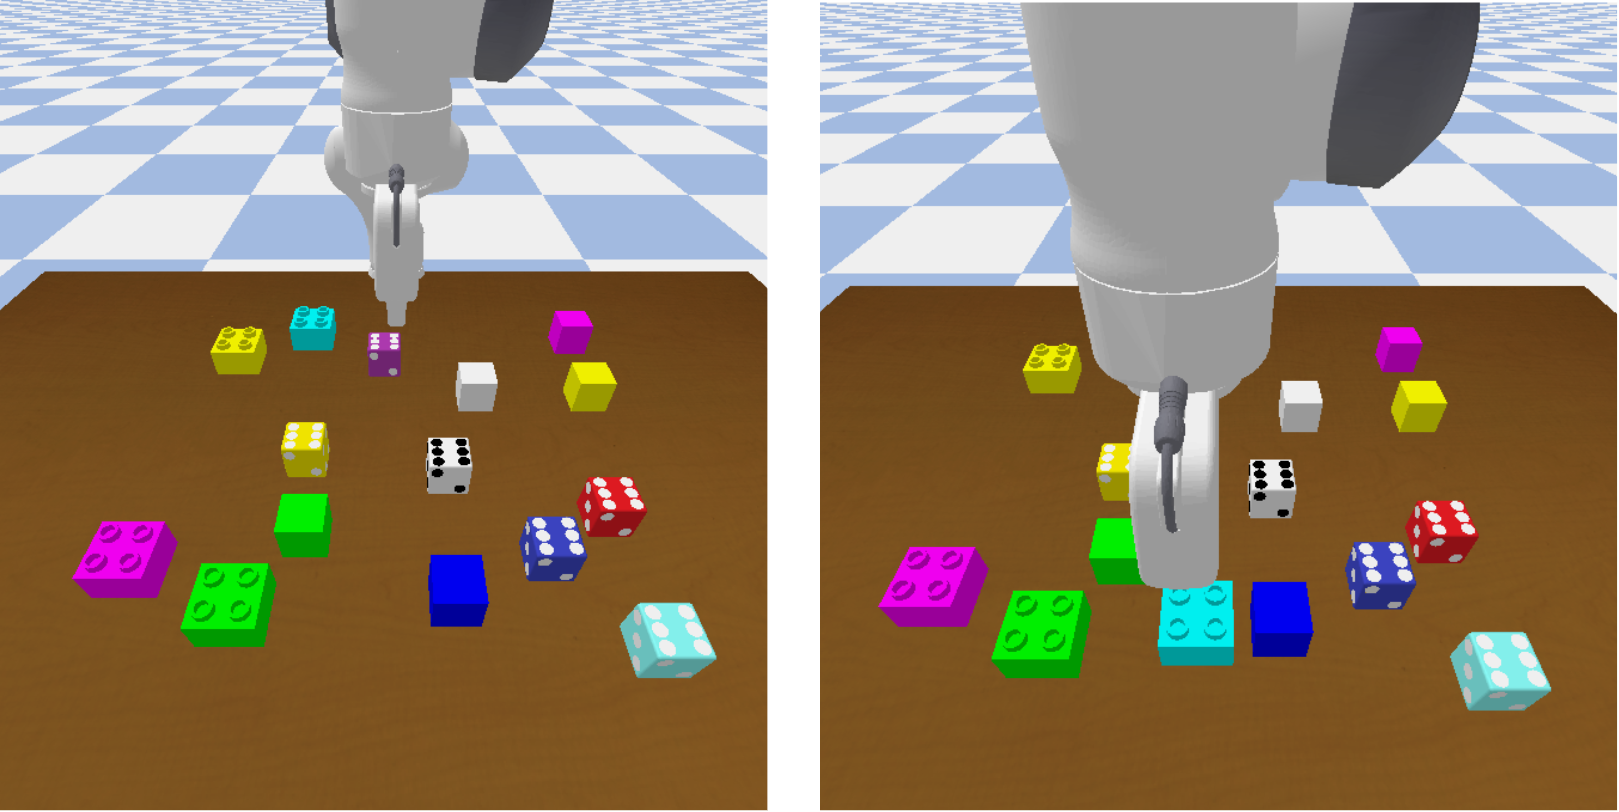
\includegraphics[width=\textwidth]{assets/qual-2.png}
        \caption{On a scene with 15 objects (Generalization to more objects), \footnotesize{"Place the cyan lego object to the left of the blue cube"}}
    \end{subfigure}
    \hfill

    \vspace{1cm}

    \begin{subfigure}{0.7\textwidth}
        \centering
        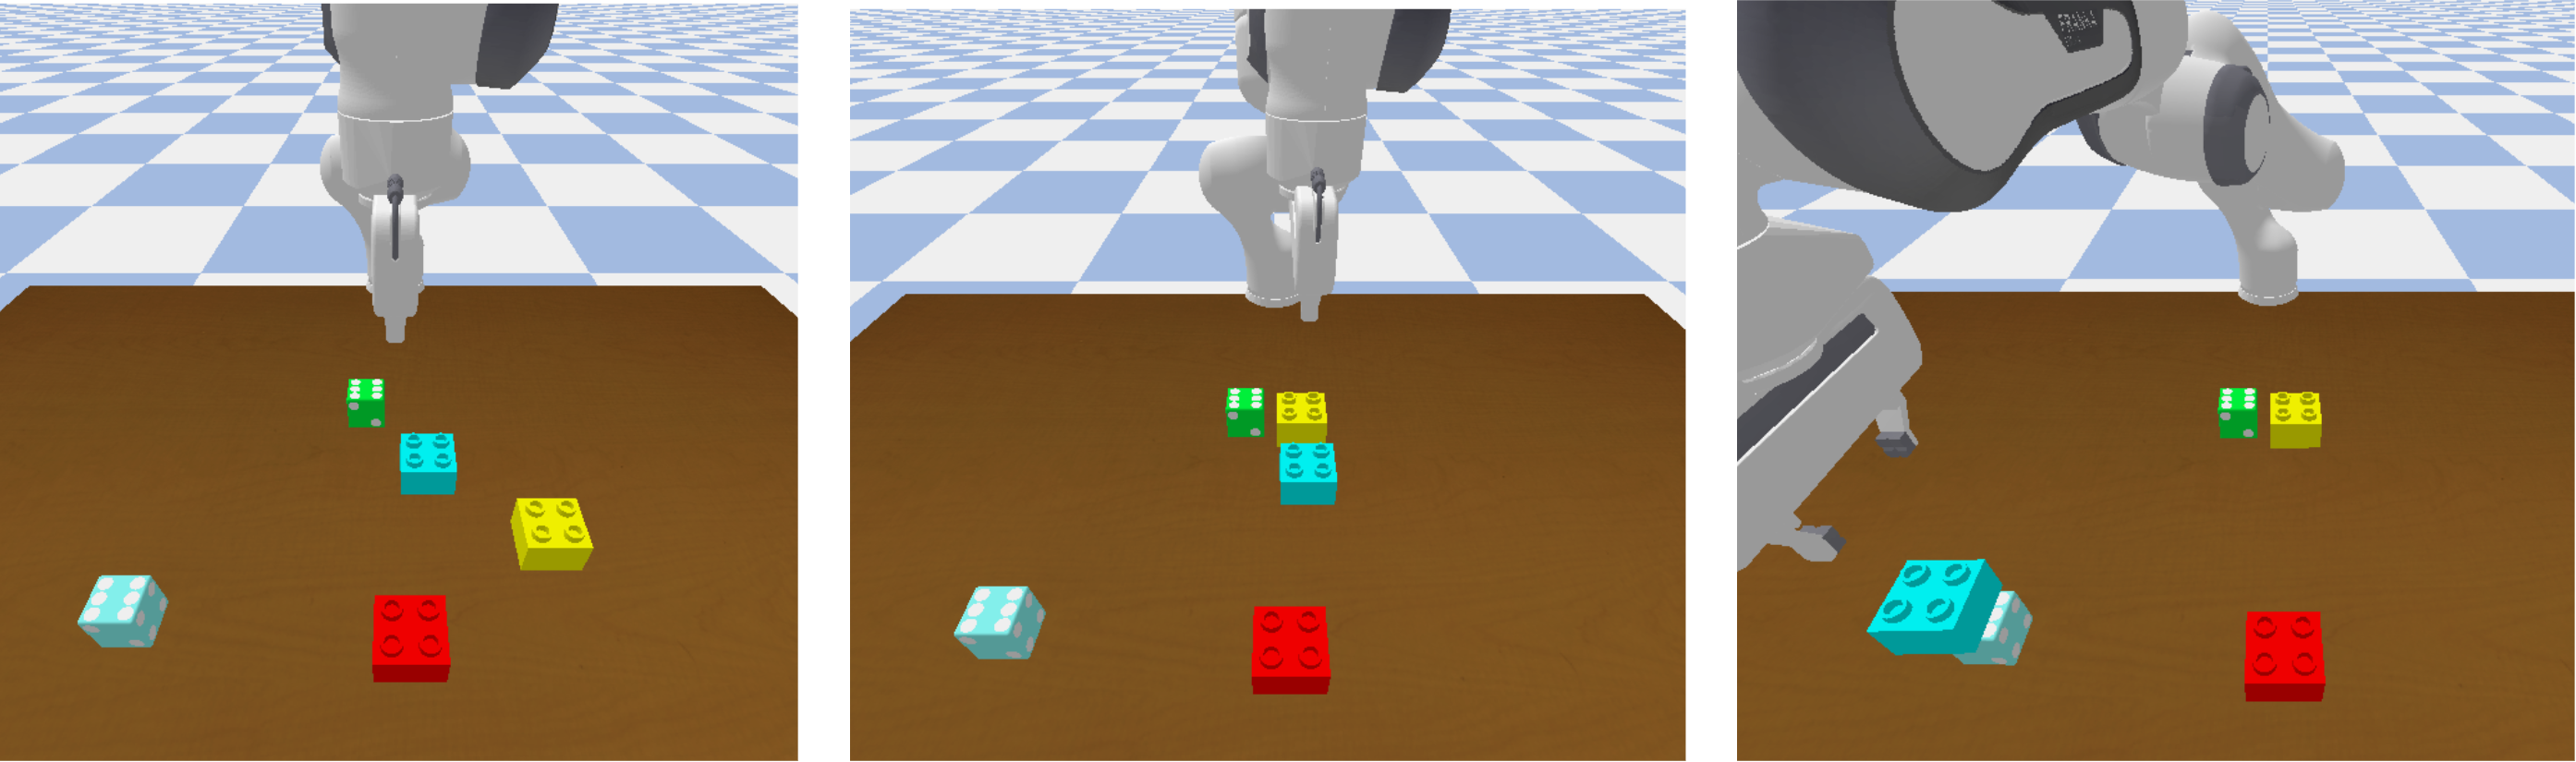
\includegraphics[width=\textwidth]{assets/qual-3.png}
        \caption{On a double step instruction with relational attributes (complex instruction), \footnotesize{"Place the thing at the right of the red lego object to the right of the green dice and put the cyan lego block on top of the cyan dice"}.}
    \end{subfigure}

    \vspace{1cm}

    \begin{subfigure}{\textwidth}
        \centering
        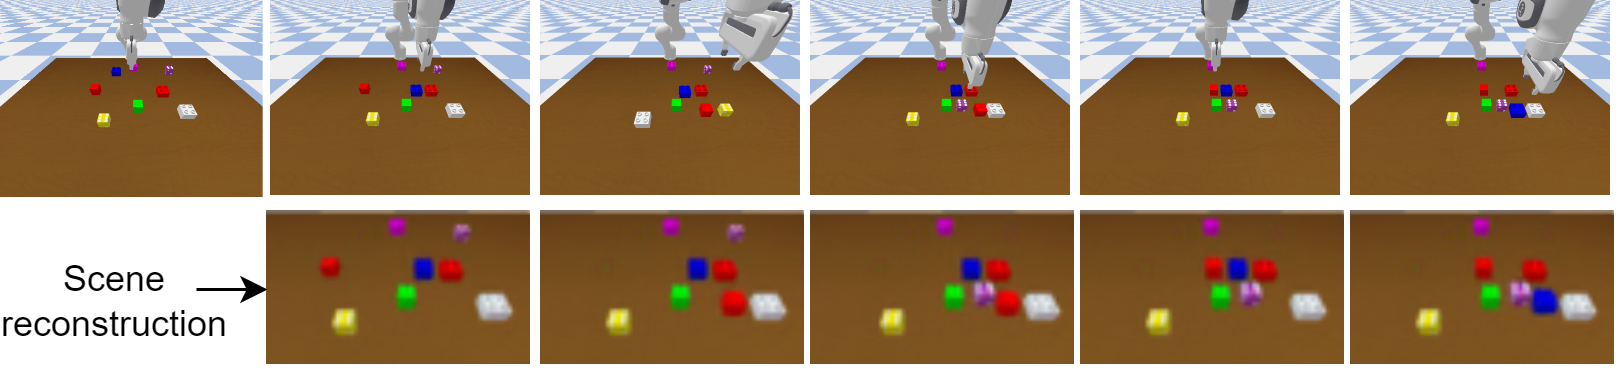
\includegraphics[width=\textwidth]{assets/qual-4.png}
        \caption{On a 5-step instruction (Generalization to longer horizon manipulation), \footnotesize{"Put the blue lego thing on the left side of the red lego thing and place the red cube on the left side of the white lego object and move the magenta dice on the right of the green box and move the red box on the left side of the blue lego thing and put the blue lego object to the left of the white lego thing"}. We Also show reconstruction of the predicted scene before each step of the simulation}
    \end{subfigure}
    
    \caption{Qualitative results of demonstration using a simulated 7-DOF manipulator}
    \label{fig:qual-1}
\end{figure}

\begin{figure}
    \centering
    \hfill
    \begin{subfigure}{0.45\textwidth}
        \centering
        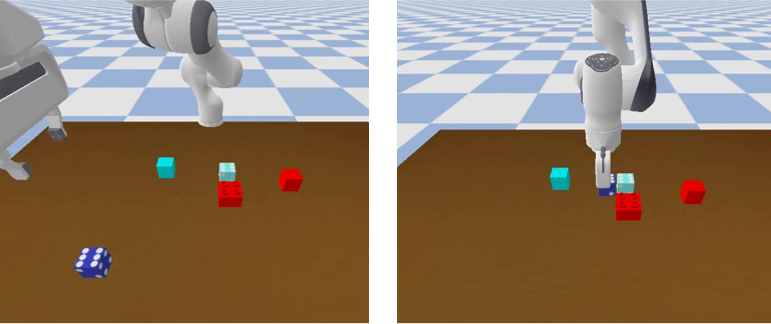
\includegraphics[width=\textwidth]{assets/cliport-qual.png}
        \caption{CLIPort: Unsuccessful execution due to incorrect grounding}
    \end{subfigure}
    \hfill
    \begin{subfigure}{0.45\textwidth}
        \centering
        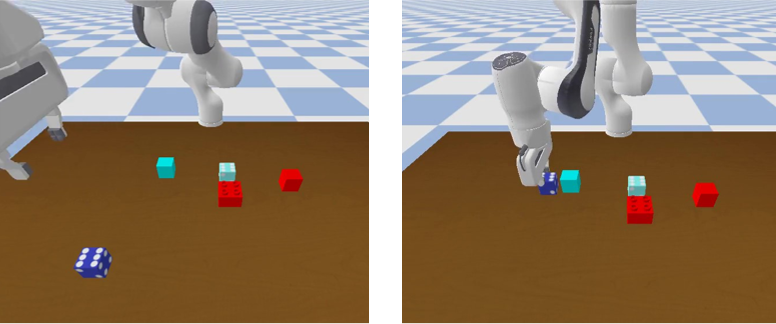
\includegraphics[width=\textwidth]{assets/cliport-qual-ours.png}
        \caption{Our model: Successful \\ execution}
    \end{subfigure}
    \hfill

    \caption{Qualitative comparison with CLIPort. Instruction: “Move the dice that is blue in color on the left side of the box which is cyan in color"}
    \label{fig:cliport-qual}
\end{figure}

\begin{figure}
    \centering
    \hfill
    \begin{subfigure}{\textwidth}
        \centering
        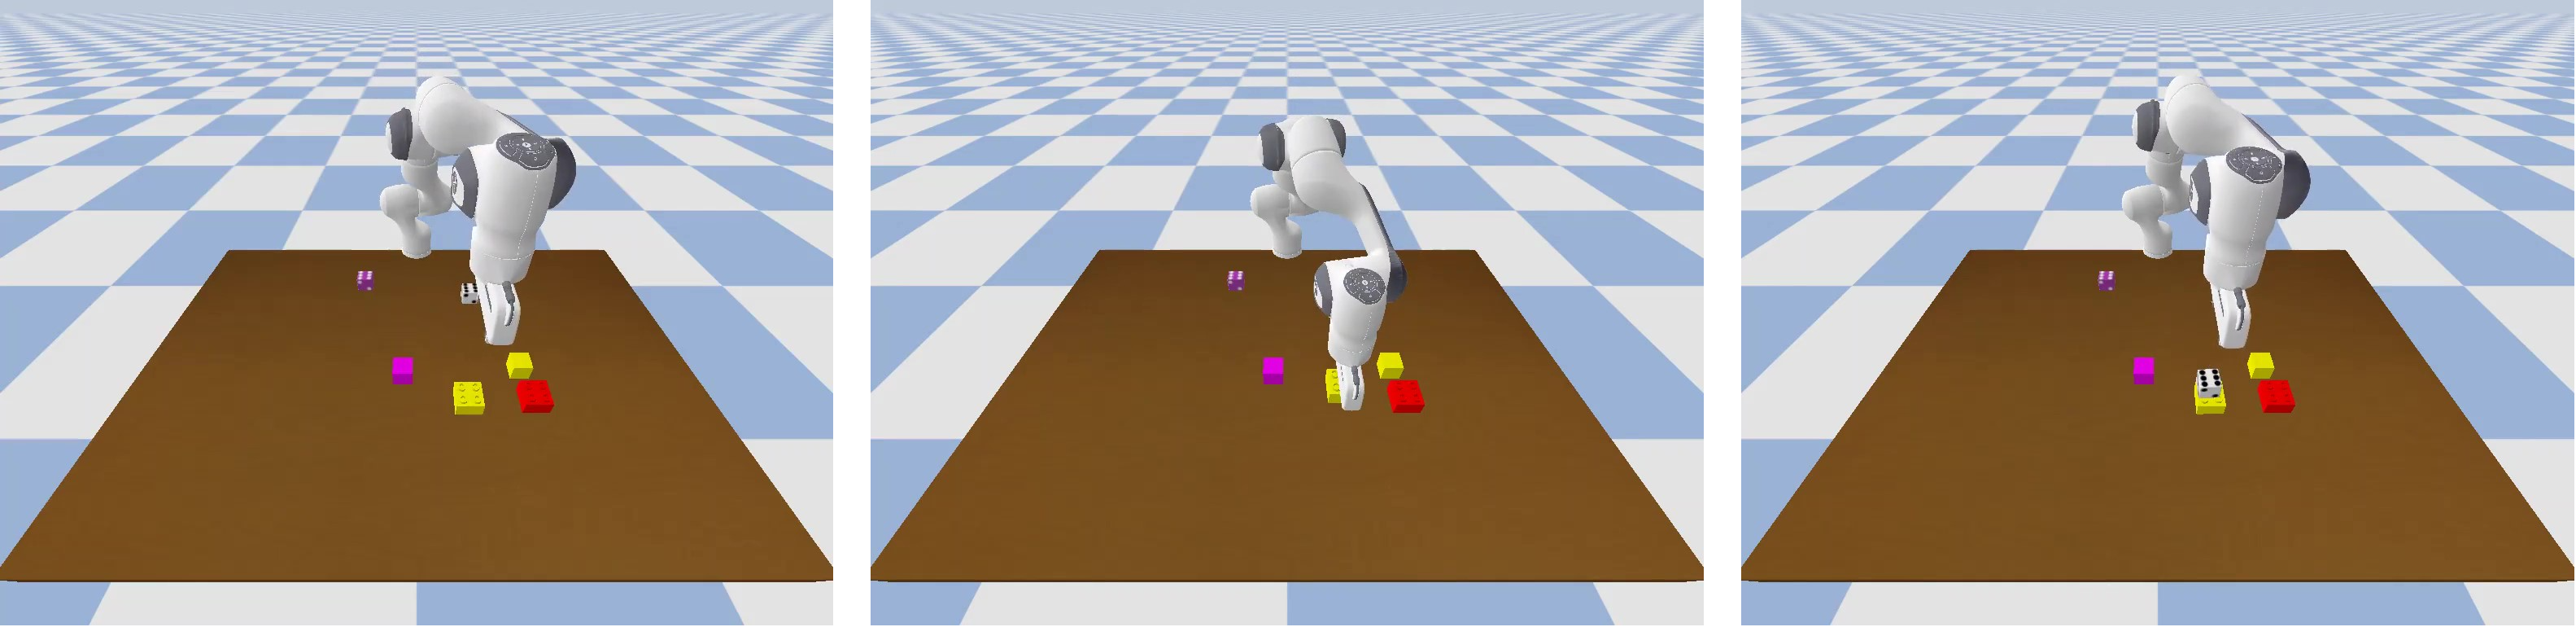
\includegraphics[width=0.9\textwidth]{assets/nmn-comb.png}
        \caption{NMN+: Unsuccessful execution due to grounding the subject and predicate objects incorrectly}
    \end{subfigure}
    \hfill
    \begin{subfigure}{\textwidth}
        \centering
        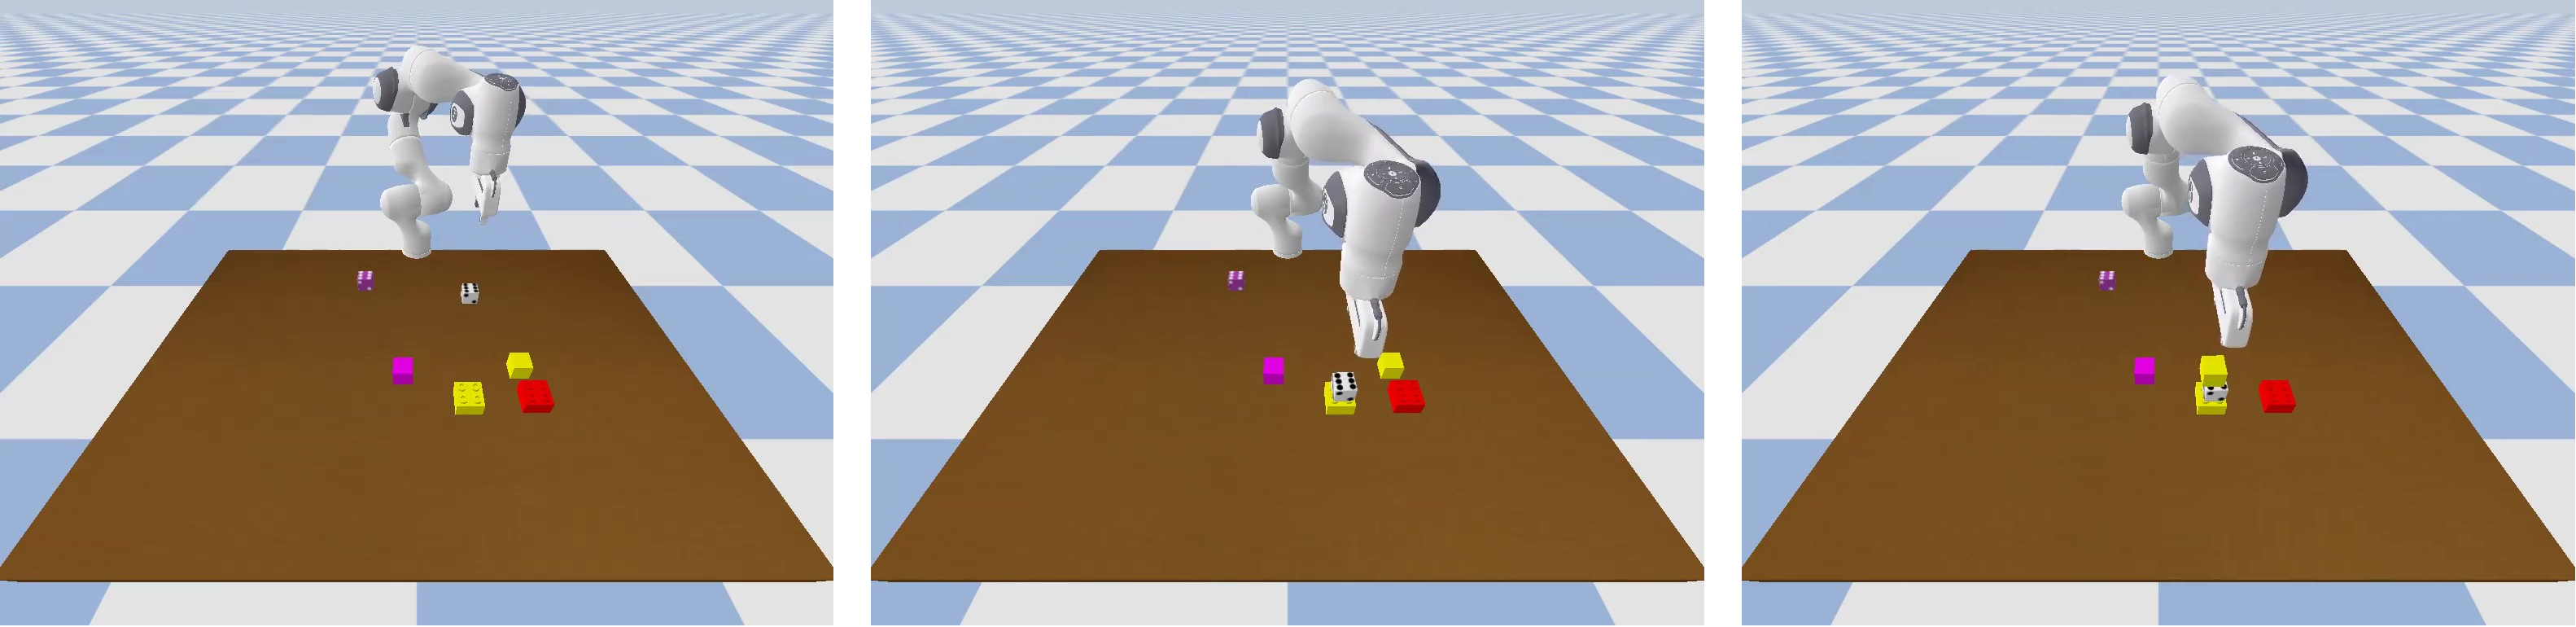
\includegraphics[width=0.9\textwidth]{assets/ours-comb.png}
        \caption{Our model: Successful \\ execution}
    \end{subfigure}
    \hfill

    \caption{Qualitative comparison with NMN+. Instruction: “Put the white dice above the yellow lego object and move the yellow cube on top of the white dice"}
    \label{fig:nmn-qual}
\end{figure}


Tables \ref{tab:accuracy} and \ref{tab:accuracy2} report the performance of our model and the baseline on the test set. We report both numbers: using gold set of bounding boxes and using bounding boxes extracted~\footnote{Excluded about 10\% no detection cases for both models.} using the approach described in subsection~\ref{subsec:visual-reason}. Our model outperforms the baseline overall. For instructions with complex reasoning (resolution of binary spatial relations) involved, the proposed model outperforms the baseline by $33$ points in the IOU-M metric. Figure~\ref{fig:nmn-qual} shows an example where our model improves over NMN+'s performance.
%
Disentangled representations of relations and concepts in \textit{Visual Reasoning} module allow the proposed model to reason over complex instructions.

\textbf{CLIPort}~\cite{shridhar2022cliport} takes as input a dense, image-based state representation, in contrast to our object-centric state representation. It proposes a two-stream architecture that computes language-guided attention masks on the input scene for both pick and place locations. It lacks explicit symbolic constructs for reasoning about the scene. Instead, the reasoning required for manipulation is performed by leveraging the visuo-linguistic understanding of the large pre-trained model CLIP ~\cite{clip}. Table ~\ref{tab:cliport} compares \emph{CLIPort} with our model. Since \emph{CLIPort} performs only single-step pick-and-place operations, the numbers are calculated only on single-step examples. The following metrics are used \begin{enumerate}
    \item \emph{Placement Accuracy}: fraction of examples in which the predicted place location lies within the groundtruth bounding box of the moved object
    \item \emph{Identification Accuracy}: fraction of examples in which the predicted pick location lies within the groundtruth bounding box of the moved object. For the proposed model, the centre of the predicted bounding box location is used as the predicted place location.
\end{enumerate}

We observe that CLIPort on our dataset shows low accuracy in both predicting the object to be moved as well as the place location. Further, its performance deteriorates in examples with relational concepts. We note that the performance and sample-efficiency of CLIPort critically depends upon  spatial consistency of input images i.e. objects do not scale or distort depending on the viewing angle as in ~\cite{shridhar2022cliport}. Figure~\ref{fig:cliport-qual} shows an example where our model improves over CLIPort's performance. To provide additional leverage to the baseline, we train CLIPort on 5 times more data than the original, results of which are reported under the title CLIPort-5x. We observe an improvement in performance on the larger dataset, although still worse than that of the proposed model. 
% This can be attributed to (i) its inability to learn from sparse dataset (due to lack of modularity), (ii) the use of raw image as state representation, and (iii) lack of spatial consistency in images, i.e. objects can scale or distort depending on the viewing angle,  in contrast to the setting used by CLIPort. To further establish CLIPort's data inefficiency, we train it with 5 times more data. Specifically, for each scene in the original dataset, we add 5 additional instructions and corresponding final scenes. This leads to improvement in performance, although inferior to that of the proposed model. 


%
%% Generalization on Larger Scenes

%% Main Results
%%%%%%%%%%%%%%%
% \subsection{Model Accuracy}
% % Quantitative evaluation
% %\textbf{Quantitative Evaluation.} 
% A quantitative evaluation of model accuracy is is carried out in two settings. First, we use a $80:20$ train:test split of the entire corpus for accuracy comparison. The corpus consists of both single step and double step commands, along with sentences of different complexities:- \textit{simple} and \textit{complex}. Complex sentences involve reasoning on inter-object relationships, while simple sentences reason over individual object features only. 




% We demonstrate our model's ability to infer a sequence of grounded sub-goals, given an initial scene and instruction, that involves manipulating the scene over multiple time step and complex multi-hop reasoning.
% %
% Table \ref{tab:accuracy} reports the performance of our model and the baseline on the test set. We report both numbers: using gold set of bounding boxes and using bounding boxes extracted~\footnote{Excluded about 10\% no detection cases for both models.} using the approach described in subsection~\ref{subsec:visual-reason}. Our model outperforms the baseline overall. For instructions with complex reasoning (resolution of binary spatial relations) involved, the proposed model outperforms the baseline by $33$ points in the IOU-M metric.
% %
% Disentangled representations of relations and concepts in \textit{Visual Reasoning} module allow the proposed model to reason over complex instructions. 

% For the remaining experiments, the numbers are reported using gold BBs for both the models.


% \texttt{Single-step} and \texttt{Double Step} refer to instructions with one and two actions involved resprectively and \texttt{Simple reasoning} refers to simple reasoning bases upon 
% reports the accuracy results. Both test (around 1700 samples) and train set (around 1700 samples) contain 1 - 2 step commands. Further, test and train do not have any 1-step command in common. Both models achieve a high accuracy during training but the proposed model shows significant improvement over the baseline for the test set.  
%
% Overall Accuracy on Test and Train Sets
%\subsection{Generalization With Increasing Scene Objects}
% The proposed model is able to interpret the correct object and move it to the correct position with marginal decline in performance to scenes with up to 10 objects after being trained on scenes with up to 5 objects only, without any obtrusive decrease in accuracy. Disentangled representations of object features and spatial features in the scene graph extracted by the \textit{Visual Reasoner} from the scene along with an object-centric view of the environment help the model to generalise strongly to larger number of objects. 


%%%%% Generalization
\subsection{Combinatorial Generalization} 

To evaluate the approaches in an out-of-distribution generalization setting, we collect dataset consisting of scenes with more objects than seen during training, and with instructions that involve larger number of steps for carrying out the task.

Figure~\ref{fig:large_scenes} illustrates the model generalizing combinatorially to scenes with more number of objects. The models were first trained on scenes having up to $5$ objects only, and then tested on scenes having up to $10$ objects.\\ 
%
The superior generalization demonstrated by the model can be attributed to reliance on an object-centric state representation and the ability to learn dense disentangled representations of spatial and action concepts, facilitating modular and structured reasoning that scales gracefully. 

Figure ~\ref{fig:large_steps} illustrates model generalization to longer horizon manipulation. We observe that the proposed model is able to perform multiple scene manipulation and reasoning steps with considerable accuracy up to $7$ steps after being trained with instructions translating to plans up to $2$ steps.\\ 
%
The performance of the object-centric baseline (NMN+) is worse and the model struggles to generalize to plans extending to longer horizons. We attribute this to the modular structure of our approach compared to the baseline.
\iffalse
\begin{figure}[h]
    \centering    
    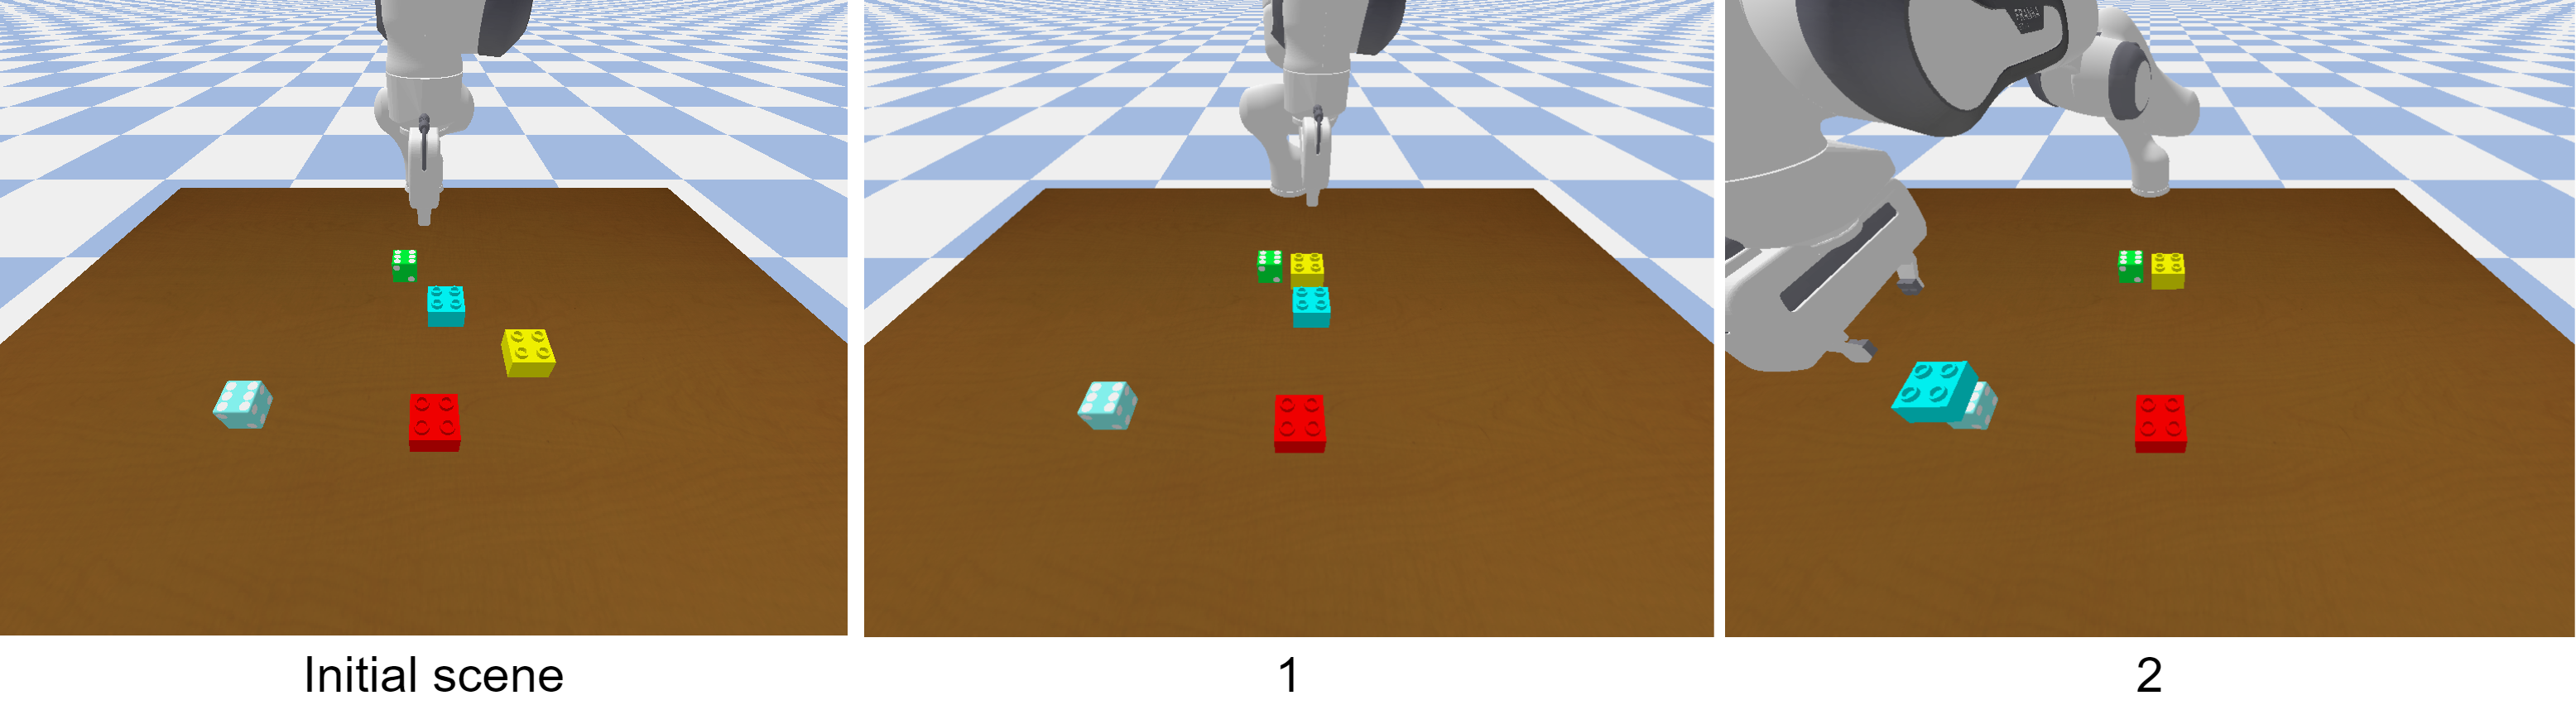
\includegraphics[width=7.5cm]{figures/rel.png}
    \caption{
    \footnotesize{Execution of robot manipulator on a double step instruction containing relational attributes: \emph{Place the thing at the right of the red lego object to the right of the green dice and put the cyan lego block on top of the cyan dice}
    }}
    \label{fig:relative}
\end{figure}
\fi
%
\subsection{Demonstration on a Simulated Robot}
%
We demonstrate the learned model for interpreting instructions 
provided to a simulated 7-DOF Franka Emika manipulator in a table top setting. 
%
The robot is provided language instructions and uses the model to predict a program that once executed transitions the world state to the intended one. The 2-D bounding boxes predicted by the action simulator are translated to 3-D coordinates in the world space via a learned MLP using simulated data.
%
The predicted positions are provided to a low-level motion planner for trajectory generation with crane grasping for picking/placing. Since there is some error in predicting exact 3-D locations from 2-D bounding boxes, the execution of the low level motion planner is improved by assuming some heuristics, preventing collisions and aligning objects on top with ones underneath.  
%Each step of the robot simulation is then performed by grasping the object at the initial location, moving the gripper to the final predicted location, and releasing the gripped object. 
% 
Figure \ref{fig:qual-1} shows execution by the robot manipulator on complex instructions, scenes having multiple objects, double step relational instructions, and multi-step instructions. 
%
Figure \ref{fig:cliport-qual} and \ref{fig:nmn-qual} show qualitative comparisons with baselines on some examples where our model improves over their performance.

We observe an execution success accuracy of 55.7\% for our model. An execution is successful if all objects are at correct positions (upto a small threshold) at each step of the instruction, and in an upright orientation. We observe that the drop in success compared to the earlier metrics is due to various reasons, such as (i) an error in bounding box predictions compounded with an error in 2D-to-3D predictions, (ii) Execution errors during grasp, release and motion trajectory during manipulation, (iii) Objects going out of range of the manipulator arm. In our next work, we adress recovery from a wide range of possible errors, including natural execution errors and manipulation by external agents. 


\subsection{Scene reconstruction}

The structural similarity index (SSIM) \cite{ssim2004} for the reconstruction model is 0.935, evaluated on the test set (containing upto 2-step instructions and upto 5 objects in the scene) by giving the ground-truth final object bounding boxes. We visualise reconstruction of the moved objects before each step of the actual execution in the 5-step instruction in figure \ref{fig:qual-1}. On further analysis, we can observe that the model correctly learns to decode the object embeddings, as can be seen in figure~\ref{fig:recons-qual}. The model is passed an empty table background as the initial input image, alongwith bounding box locations and embeddings of all objects. Switching all object colours to blue also yields the correct scene, demonstrating generalization to unseen combinations. 


\begin{figure}
    \centering

    \hfill
    \begin{subfigure}{0.24\textwidth}
        \centering
        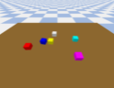
\includegraphics[width=\textwidth]{assets/recons-gt.png}
        \caption{Ground-truth final scene\\ \\ \\}
    \end{subfigure}
    \hfill
    \begin{subfigure}{0.24\textwidth}
        \centering
        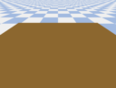
\includegraphics[width=\textwidth]{assets/recons-init.png}
        \caption{Initial empty bg image passed to the model with object embeddings and bboxes}
    \end{subfigure}
    \hfill
    \begin{subfigure}{0.24\textwidth}
        \centering
        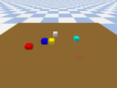
\includegraphics[width=\textwidth]{assets/recons-recon.png}
        \caption{Reconstructed final scene \\ \\ \\}
    \end{subfigure}
    \hfill
    \begin{subfigure}{0.24\textwidth}
        \centering
        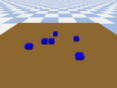
\includegraphics[width=\textwidth]{assets/recons-blue.png}
        \caption{Reconstructed scenes if all object types are changed to blue \\}
    \end{subfigure}
    \hfill
    
    \caption{Qualitative analysis of scene reconstruction}
    \label{fig:recons-qual}
\end{figure}



\iffalse
\subsection{Failure cases}
In roughly 10\% of examples in the dataset, the object detector returns a false object proposal, or misses an object, in either of initial or final scenes. Since we are unable to calculate loss in such cases, these examples are not considered for experiments with perception.
\fi

%%%% ATTIC %%%%
\iffalse

% Table~\ref{tab:accuracy} reports the performance of our model and the baseline on the test set. 
% reports the accuracies for the proposed and the 
% baseline models. The results indicate a stronger generalization for the proposed approach compared to the baseline model.
%
% The result illustrates the model’s ability to reason about language instructions with novel object attribute references in the context of the scene. Such visual-linguistic reasoning operates on a single scene. Next, we assess generalization over multiple time steps. We explicitly evaluate the model on a test cases where an instruction involves multi-step actions that exceed those seen in training.

% %  \vspace{-2em}
% \begin{table}
%     \centering
%     \caption{Generalization On Instructions with Novel Object Attributes}
%     \begin{tabular}{|c|c|c|c|c|c|c|c|}
%     \hline
%     Model & Prog ($P$) & Arg ($O_1$) & Arg ($O_2$) & IOU-2D & IOU-3D \\ \hline \hline
%     Baseline & - & 87.5 & 89.1 & 29.0 & 16.6 \\ 
%     Ours &  98.5 & 96.3 & 96.3 & 51.6  & 25.2  \\
%    \hline
%     \end{tabular}
%     \label{tab:generalization-attributes}
% \end{table}
% %
%  \vspace{-0.5em}
% \begin{table}
%     \centering
%     \caption{Generalization over Three-step Instructions with One/Two-step Instructions in Training}
%     \begin{tabular}{|c|c|c|c|c|c|}
%     \hline
%     %Model &$P$ & ($P_g$) & ($o_1$) & ($o_2$) & IOU-2D & IOU-3D \\ 
%     Model & Prog ($P$) & Arg ($O_1$) & Arg ($O_2$) & IOU-2D & IOU-3D \\
%     \hline \hline
%     Baseline & - & 76.0  & 80.9 & 13.3 &  6.6  \\
%     Our & 56.8  & 54.7 & 53.6 & 27.2 & 12.9 \\
%     % Random & 12.5 & 0.09 & 3.4 & 3.4 & - & -\\
%     \hline
%     \end{tabular}
%     \label{tab:generalization-multi-step}
% \end{table}

% Table~\ref{tab:generalization-multi-step} presents the results. The models were only trained on 1-2 step commands, and are tested on 3 step commands. The proposed model shows improved generalization compared to the baseline in the IOU metrics. 

% %  \vspace{-2em}
% \begin{table}
%     \centering
%     \caption{Generalization to Novel Multi-Object Attribute Instructions}
%     \begin{tabular}{|c|c|c|c|c|c|}
%     \hline
%         Model & Prog ($P$) & Arg ($O_1$) & Arg ($O_2$) & IOU-2D & IOU-3D \\\hline \hline
%         %Model & ($P$) & ($o_1$) & ($o_2$) & IOU-2D & IOU-3D \\  \hline \hline
%         Baseline & - &55.0 &32.4 & 3.2& 1.5\\
%       Ours & 98.0 & 75.7 & 89.5 & 27.3 & 9.3 \\ \hline 
%     %   Baseline & 84.3 & 90.2 & 93.0 & 49.0 & 30.3     \\\hline
%     \end{tabular}
%     % \vspace{1em}
    \label{tab:generalization-multiple-object-attributes}
% \end{table}

% Table~\ref{tab:generalization-multiple-object-attributes} presents evaluation on task instructions that involve multi-step reasoning over attributes in the setting where the model is trained 
% only on a single attribute. For example, the training set instructions only involve singe 
% attributes such as 'red' and 'lego' with two different objects but during testing the model must compositional reason over both attributes to understand and follow the instruction. As before, 
% the ability to combine grounded concepts with reasoning allows the proposed model to generalize 
% better in this setting achieving significantly higher generalization accuracy compared to the baseline. 

% The above results demonstrate stronger generalization to novel scenes with unseen object attribute pairs as well as action sequences that extend beyond those encountered during training. 
% %
% The neuro-symbolic approach involves learning of data-driven learning of concept representations that are amenable to rich compositional reasoning. The neuro-symbolic approach transfers better to novel settings compared to the direct neural-only approach that does not make use of the modular structure during training.

\begin{figure}[ht]
    \centering
    \setlength\tabcolsep{1.5pt}
    \begin{tabular}{ccc}
      \includegraphics[width=28mm]{figures/1step/rgba0002.png} &   \includegraphics[width=28mm]{figures/1step/rgba0009.png} &
      \includegraphics[width=28mm]{figures/1step/rgba0017.png}\\
    % \multicolumn{2}{c}{\includegraphics[width=55mm]{it} }\\
    % \multicolumn{2}{c}{(e) fifth}
    \end{tabular}
    \caption{A robot manipulator correctly performing a single step instruction \emph{``put cyan block on blue block"} in a simulated table top environment. }
    \label{fig:demo-1}
\end{figure}

%
Figure~\ref{fig:demo-1} illustrates the robot successfully performing a single step instruction, \emph{``put cyan block on the blue block"} using the sub-goal predicted by the inferred program. 

%
Figure~\ref{fig:demo-2} illustrates the robot manipulator performing the instruction \emph{``put yellow block to the left of white block and put magenta small block on yellow block"}. the model reasons about the input instruction in the context of the environment correctly positions the yellow block on the left side of the intended white block. Subsequently, the robot grasps the magenta block and correctly positions the block on the yellow block that was previously manipulated. 

\begin{figure}
    \centering
    \setlength\tabcolsep{1.5pt}
    \begin{tabular}{ccc}
       \includegraphics[trim={5cm 5cm 5cm 0},clip,width=28mm]{figures/2step_s/rgba0002.png}  &
       \includegraphics[trim={5cm 5cm 5cm 0},clip,width=28mm]{figures/2step_s/rgba0006.png}  &
       \includegraphics[trim={5cm 5cm 5cm 0},clip,width=28mm]{figures/2step_s/rgba0011.png} \\
       \includegraphics[trim={5cm 5cm 5cm 0},clip,width=28mm]{figures/2step_s/rgba0015.png} &
       \includegraphics[trim={5cm 5cm 5cm 0},clip,width=28mm]{figures/2step_s/rgba0020.png} &
       \includegraphics[trim={5cm 5cm 5cm 0},clip,width=28mm]{figures/2step_s/rgba0021.png} 
    \end{tabular}
    \caption{Robot manipulator performing a two-step instruction \emph{``put yellow block to the left of white block and put magenta small block on yellow block"}}
    \label{fig:demo-2}
\end{figure}
%Further, note that the model used in the demonstrates shown in 
%Figures~\ref{fig:demo-2} and~\ref{fig:demo-2} 

% Incorrect: multi step instruction. 
\begin{figure}
    \centering
    \setlength\tabcolsep{1.5pt}
    \begin{tabular}{ccc}
       \includegraphics[trim={5cm 5cm 5cm 0},clip,width=28mm]{figures/2step_f/rgba0002.png}  &  
       \includegraphics[trim={5cm 5cm 5cm 0},clip,width=28mm]{figures/2step_f/rgba0008.png}  &
       \includegraphics[trim={5cm 5cm 5cm 0},clip,width=28mm]{figures/2step_f/rgba0016.png} \\
       \includegraphics[trim={5cm 5cm 5cm 0},clip,width=28mm]{figures/2step_f/rgba0026.png} &
       \includegraphics[trim={5cm 5cm 5cm 0},clip,width=28mm]{figures/2step_f/rgba0031.png} &
       \includegraphics[trim={5cm 5cm 5cm 0},clip,width=28mm]{figures/2step_f/rgba0034.png} \\
    %   \multicolumn{3}{c}{Robot manipulator performing a double step instruction \emph{"put red block on blue block and put magenta block on red block"}. The robot correctly inferred the sequence of symbolic actions but failed during execution error due to the unstable placement of the second block. }
    \end{tabular}
    \caption{Robot manipulator performing a two-step instruction \emph{"put red block on blue block and put magenta block on red block"}. The robot correctly inferred the sequence of symbolic actions but failed during execution error due to the unstable placement of the second block. }
    \label{fig:demo-3}
\end{figure}

%
Figure~\ref{fig:demo-3} shows the execution for the instruction \emph{``put red block on blue block and put magenta block on red block"}. The model correctly predicts a program consisting of a composition of two sequential manipulation actions. The robot correctly identifies the intended objects for manipulation, then grasps and re-positions them to form the intended assembly. In the final step, the robot correctly placed the magenta-colored block on top of the red-colored block, however, the inferred placement was unstable and the block fell from the assembly. Note that the current model infers the task plan which is then handed over to the motion planner. Such a staged approach possesses the inherent limitation of not being able to recover from execution failures. The possibilities of a reactive approach by interleaving planning and execution are to be explored in future work and is likely to benefit error-recovery.

%
In Figure~\ref{fig:demo-4}, the robot is provided with the instruction, \emph{``put red block to the left of yellow block and put cyan block to the left of red block and then put red block on cyan block"} which requires three successive manipulations. The model used in this experiment is trained only on two step instructions. However, at inference time, the model can generalize to a longer instruction by leveraging the compositionality inherent in our program representation. 


\begin{figure}
    \centering
    \setlength\tabcolsep{1.5pt}
    \begin{tabular}{ccc}
       \includegraphics[trim={5cm 5cm 5cm 0},clip,width=28mm]{figures/3step_s/rgba0002.png} &  
       \includegraphics[trim={5cm 5cm 5cm 0},clip,width=28mm]{figures/3step_s/rgba0011.png}  &
       \includegraphics[trim={5cm 5cm 5cm 0},clip,width=28mm]{figures/3step_s/rgba0015.png} \\
       \includegraphics[trim={5cm 5cm 5cm 0},clip,width=28mm]{figures/3step_s/rgba0020.png} &
       \includegraphics[trim={5cm 5cm 5cm 0},clip,width=28mm]{figures/3step_s/rgba0025.png} &
       \includegraphics[trim={5cm 5cm 5cm 0},clip,width=28mm]{figures/3step_s/rgba0030.png} \\
    \end{tabular}
    \caption{Robot manipulator performing a three-step instruction \emph{``put red block to the left of yellow block and put cyan block to the left of red block and then put red block on cyan block"}. The robot correctly inferred the sequence of actions. }
    \label{fig:demo-4}
\end{figure}
\fi


% \begin{figure*}[hbt!]
%     \centering    
%     \includegraphics[width=15cm]{figures/qualitative.png}
%     \caption{
%     \footnotesize{Execution of robot manipulator on a 5-step instruction: \emph{Put the blue lego thing on the left side of the red lego thing and place the red cube on the left side of the white lego object and move the magenta dice to the right of the green box and move the red box on the left side of the blue lego thing and put the blue lego object to the left of the white lego thing}. The first row shows the scene after each action in the robot simulation. The second row shows reconstruction of the predicted scene before each step of the simulation
%     }}
%     \label{fig:qualitative}
% \end{figure*}

\section{Conclusion}\label{sec:conclusion}
We present a discrepancy-aware neuro-symbolic approach for plan recovery from failures. Unlike existing approaches, we do not require hand-annotated data of failures, rather we make use of self-supervision to train our recovery model. %, rather we make use of self-supervision to learn our underlying failure discovery and recovery mechanism. 
Our approach makes use of object-centric representation of the state in the form a dense scene-graph. We train neural modules to learn the transition function based on data gathered from an existing neuro-symbolic planner. Additionally, we train neural discriminators, trained via the help other states encountered during execution as negatives, to help us distinguish the representations of the simulated state (desired) from the failure states. Once a failure is detected, a recovery plan is constructed to join back the originally constructed plan at an appropriate point. 
%Directions for future work include working with partial observability during plan execution, and dealing with more complex failure scenarios such as objects dis-appearing from the scene, e.g., falling off the table.
\section{Acknowledgements}
%We thank IIT Delhi HPC facility\footnote{\emph{http://supercomputing.iitd.ac.in}} for computational resources. 
We thank anonymous reviewers for their insightful comments that helped in further improving our paper.
Parag Singla was supported by the DARPA Explainable AI (XAI) Program,
%with number \#N66001-17-2-4032, 
IBM AI Horizon Networks (AIHN) grant and
%the Visvesvaraya Young Faculty Fellowships by Govt. of India and 
IBM SUR awards.
Rohan Paul acknowledges Pankaj Gupta Young Faculty Fellowship for support. 
%This work was partially supported by the CSE Research Acceleration fund of IIT Delhi. 
We acknowledge the support of CSE Research Acceleration fund of IIT Delhi. Any opinions, findings, conclusions or recommendations
expressed in this paper are those of the authors and do
not necessarily reflect the views or official policies, either expressed or implied, of the funding agencies.

%\bibliographystyle{iEEEtranS.bst}

%{ieeeconf}
\newpage
\printbibliography

\end{document}



%authors 
%add main equation 
%